\documentclass[spanish,]{book}
\usepackage{lmodern}
\usepackage{amssymb,amsmath}
\usepackage{ifxetex,ifluatex}
\usepackage{fixltx2e} % provides \textsubscript
\ifnum 0\ifxetex 1\fi\ifluatex 1\fi=0 % if pdftex
  \usepackage[T1]{fontenc}
  \usepackage[utf8]{inputenc}
\else % if luatex or xelatex
  \ifxetex
    \usepackage{mathspec}
  \else
    \usepackage{fontspec}
  \fi
  \defaultfontfeatures{Ligatures=TeX,Scale=MatchLowercase}
\fi
% use upquote if available, for straight quotes in verbatim environments
\IfFileExists{upquote.sty}{\usepackage{upquote}}{}
% use microtype if available
\IfFileExists{microtype.sty}{%
\usepackage{microtype}
\UseMicrotypeSet[protrusion]{basicmath} % disable protrusion for tt fonts
}{}
\usepackage{hyperref}
\hypersetup{unicode=true,
            pdftitle={Fundamentos de Investigación II},
            pdfauthor={Luis Eudave},
            pdfborder={0 0 0},
            breaklinks=true}
\urlstyle{same}  % don't use monospace font for urls
\ifnum 0\ifxetex 1\fi\ifluatex 1\fi=0 % if pdftex
  \usepackage[shorthands=off,main=spanish]{babel}
\else
  \usepackage{polyglossia}
  \setmainlanguage[]{spanish}
\fi
\usepackage{natbib}
\bibliographystyle{apalike}
\usepackage{color}
\usepackage{fancyvrb}
\newcommand{\VerbBar}{|}
\newcommand{\VERB}{\Verb[commandchars=\\\{\}]}
\DefineVerbatimEnvironment{Highlighting}{Verbatim}{commandchars=\\\{\}}
% Add ',fontsize=\small' for more characters per line
\usepackage{framed}
\definecolor{shadecolor}{RGB}{248,248,248}
\newenvironment{Shaded}{\begin{snugshade}}{\end{snugshade}}
\newcommand{\KeywordTok}[1]{\textcolor[rgb]{0.13,0.29,0.53}{\textbf{#1}}}
\newcommand{\DataTypeTok}[1]{\textcolor[rgb]{0.13,0.29,0.53}{#1}}
\newcommand{\DecValTok}[1]{\textcolor[rgb]{0.00,0.00,0.81}{#1}}
\newcommand{\BaseNTok}[1]{\textcolor[rgb]{0.00,0.00,0.81}{#1}}
\newcommand{\FloatTok}[1]{\textcolor[rgb]{0.00,0.00,0.81}{#1}}
\newcommand{\ConstantTok}[1]{\textcolor[rgb]{0.00,0.00,0.00}{#1}}
\newcommand{\CharTok}[1]{\textcolor[rgb]{0.31,0.60,0.02}{#1}}
\newcommand{\SpecialCharTok}[1]{\textcolor[rgb]{0.00,0.00,0.00}{#1}}
\newcommand{\StringTok}[1]{\textcolor[rgb]{0.31,0.60,0.02}{#1}}
\newcommand{\VerbatimStringTok}[1]{\textcolor[rgb]{0.31,0.60,0.02}{#1}}
\newcommand{\SpecialStringTok}[1]{\textcolor[rgb]{0.31,0.60,0.02}{#1}}
\newcommand{\ImportTok}[1]{#1}
\newcommand{\CommentTok}[1]{\textcolor[rgb]{0.56,0.35,0.01}{\textit{#1}}}
\newcommand{\DocumentationTok}[1]{\textcolor[rgb]{0.56,0.35,0.01}{\textbf{\textit{#1}}}}
\newcommand{\AnnotationTok}[1]{\textcolor[rgb]{0.56,0.35,0.01}{\textbf{\textit{#1}}}}
\newcommand{\CommentVarTok}[1]{\textcolor[rgb]{0.56,0.35,0.01}{\textbf{\textit{#1}}}}
\newcommand{\OtherTok}[1]{\textcolor[rgb]{0.56,0.35,0.01}{#1}}
\newcommand{\FunctionTok}[1]{\textcolor[rgb]{0.00,0.00,0.00}{#1}}
\newcommand{\VariableTok}[1]{\textcolor[rgb]{0.00,0.00,0.00}{#1}}
\newcommand{\ControlFlowTok}[1]{\textcolor[rgb]{0.13,0.29,0.53}{\textbf{#1}}}
\newcommand{\OperatorTok}[1]{\textcolor[rgb]{0.81,0.36,0.00}{\textbf{#1}}}
\newcommand{\BuiltInTok}[1]{#1}
\newcommand{\ExtensionTok}[1]{#1}
\newcommand{\PreprocessorTok}[1]{\textcolor[rgb]{0.56,0.35,0.01}{\textit{#1}}}
\newcommand{\AttributeTok}[1]{\textcolor[rgb]{0.77,0.63,0.00}{#1}}
\newcommand{\RegionMarkerTok}[1]{#1}
\newcommand{\InformationTok}[1]{\textcolor[rgb]{0.56,0.35,0.01}{\textbf{\textit{#1}}}}
\newcommand{\WarningTok}[1]{\textcolor[rgb]{0.56,0.35,0.01}{\textbf{\textit{#1}}}}
\newcommand{\AlertTok}[1]{\textcolor[rgb]{0.94,0.16,0.16}{#1}}
\newcommand{\ErrorTok}[1]{\textcolor[rgb]{0.64,0.00,0.00}{\textbf{#1}}}
\newcommand{\NormalTok}[1]{#1}
\usepackage{longtable,booktabs}
\usepackage{graphicx,grffile}
\makeatletter
\def\maxwidth{\ifdim\Gin@nat@width>\linewidth\linewidth\else\Gin@nat@width\fi}
\def\maxheight{\ifdim\Gin@nat@height>\textheight\textheight\else\Gin@nat@height\fi}
\makeatother
% Scale images if necessary, so that they will not overflow the page
% margins by default, and it is still possible to overwrite the defaults
% using explicit options in \includegraphics[width, height, ...]{}
\setkeys{Gin}{width=\maxwidth,height=\maxheight,keepaspectratio}
\IfFileExists{parskip.sty}{%
\usepackage{parskip}
}{% else
\setlength{\parindent}{0pt}
\setlength{\parskip}{6pt plus 2pt minus 1pt}
}
\setlength{\emergencystretch}{3em}  % prevent overfull lines
\providecommand{\tightlist}{%
  \setlength{\itemsep}{0pt}\setlength{\parskip}{0pt}}
\setcounter{secnumdepth}{5}
% Redefines (sub)paragraphs to behave more like sections
\ifx\paragraph\undefined\else
\let\oldparagraph\paragraph
\renewcommand{\paragraph}[1]{\oldparagraph{#1}\mbox{}}
\fi
\ifx\subparagraph\undefined\else
\let\oldsubparagraph\subparagraph
\renewcommand{\subparagraph}[1]{\oldsubparagraph{#1}\mbox{}}
\fi

%%% Use protect on footnotes to avoid problems with footnotes in titles
\let\rmarkdownfootnote\footnote%
\def\footnote{\protect\rmarkdownfootnote}

%%% Change title format to be more compact
\usepackage{titling}

% Create subtitle command for use in maketitle
\providecommand{\subtitle}[1]{
  \posttitle{
    \begin{center}\large#1\end{center}
    }
}

\setlength{\droptitle}{-2em}

  \title{Fundamentos de Investigación II}
    \pretitle{\vspace{\droptitle}\centering\huge}
  \posttitle{\par}
    \author{Luis Eudave}
    \preauthor{\centering\large\emph}
  \postauthor{\par}
      \predate{\centering\large\emph}
  \postdate{\par}
    \date{2020-10-15}

\usepackage{booktabs}
\usepackage{longtable}

\begin{document}
\maketitle

{
\setcounter{tocdepth}{1}
\tableofcontents
}
\chapter{Introducción a la probabilidad}\label{probability}

Para muchas personas, cuando piensan en estadística se les viene esto a
la mente: calcular promedios, recopilar datos, elaborar gráficos y
ponerlos todos en un informe en algún lugar. Mas o menos como
coleccionar sellos o cucharillas, pero con números. Sin embargo, las
estadística cubre mucho más que eso. De hecho, la estadística
descriptiva es una de las partes más pequeñas de la estadística, y una
de las menos poderosas (en cuanto a las conclusiones que puede aportar).
La parte más importante y más útil de la estadística es aquella que que
permite hacer \emph{inferencias} sobre los datos.

Una vez contemplada las estadística en estos términos, -que la
estadística está ahí para ayudarnos a hacer inferencias a partir de
datos- podemos ver ejemplos de ella en todas partes. Por ejemplo, aquí
hay un pequeño extracto de un periódico mexicano:

\begin{quote}
``Tengo un trabajo difícil'', dijo el Presidente mexicano en respuesta a
una encuesta que encontró que su gobierno ha pasado de gozar los mayores
índices de popularidad en la historia (\textgreater{}70\%) a un 38 por
ciento.
\end{quote}

Este tipo de comentarios suele pasar como completamente irrelevante en
los periódicos o en la vida cotidiana, pero pensemos brevemento sobre lo
que implica. Una compañía encuestadora ha realizado una encuesta,
presumiblemente una muy grande porque tiene los medios y puede
permitírselo. Imaginemos que llamaron a 1.000 votantes al azar, y 380
(38\%) de ellos afirmaron que tenían la intención de votar por el
Presidente. En las últimas elecciones federals, la Instituto Electoral
Mexicano confirmó la participación de 56.611.027 votantes; por lo tanto,
las opiniones de los 56.610.027 votantes restantes (aproximadamente el
99.998\% de los votantes) siguen siendo desconocidas para la
encuestadora (y para nosotros). Aún suponiendo que nadie mintió en la
encuesta, lo único que podemos decir con un 100\% de seguridad es que el
verdadero voto primario al Presidente está en algún lugar entre
380/56.611.027 (aproximadamente el 0.0007\%) y 56.610.307/56.611.027
(alrededor del 99.9987\%), lo cual no aporta mucho. Entonces, ¿sobre qué
base es legítimo para la empresa encuestadora, el periódico y el
lectores concluir que la intención de voto al Presidente mexicano fue de
sólo el 38\%?

La respuesta a la pregunta es bastante obvia: si llamo a 1.000 personas
al azar, y 380 de ellas dicen tienen la intención de votar por el
Presidente, entonces parece muy poco probable que estas sean las
\emph{únicas} 380 personas del todo el público votante que realmente
tiene la intención de hacerlo. En otras palabras, suponemos que los
datos recopilados por la empresa encuestadora son bastante
representativos de la población en general. ¿Pero qué tan
representativo? ¿Nos sorprendería descubrir que la verdadera intención
de voto es en realidad del 34\%? ¿39\%? ¿57\%? En este punto nuestración
intuición comienza a romperse un poco. Nadie se sorprendería si fuese el
34\%, y todos lo harían con un 57\%, pero es un poco difícil decir si el
39\% es plausible. Necesitamos herramientas más poderosas que solo el
mirar los números y adivinar.

\textbf{\emph{La estadística inferencial}} proporciona las herramientas
que necesitamos para responder a este tipo de preguntas, y ya que este
tipo de preguntas se encuentran en el corazón del quehacer científico,
ocupan una parte sustancial de cada curso introductorio sobre
estadística y métodos de investigación. Sin embargo, la teoría sobre la
estadística inferencial está construida sobre la \textbf{\emph{teoría de
probabilidad}}. Y es a la teoría de la probabilidad a la que ahora
debemos prestar atención. La discusión de la teoría de la probabilidad
en esta asignatura será básicamente de fondo: no hay mucho contenido
estadístico \emph{per se} en este capítulo. Sin embargo, debido a que
gran parte de la estadística se sustenta en la teoría de la
probabilidad, merece la pena ir cubriendo algunos de los conceptos
básicos.

\section{¿Cómo de diferentes son la probabilidad y la
estadística?}\label{probstats}

Antes de comenzar a hablar sobre la teoría de la probabilidad, es útil
pensar un momento en la relación que existe entre probabilidad y
estadística. Las dos disciplinas están estrechamente relacionadas, pero
no son idénticas. La teoría de la probabilidad es ``la doctrina de las
posibilidades''. Es una rama de las matemáticas que te dice con qué
frecuencia sucederán diferentes tipos de eventos. Por ejemplo, todas
estas preguntas son cosas que puedes responder usando la teoría de la
probabilidad:

\begin{itemize}
\tightlist
\item
  ¿Cuáles son las probabilidades de que al lanzar una moneda salga cara
  10 veces seguidas?
\item
  Si lanzo dos dados de seis caras, ¿qué probabilidad hay de que tire
  dos seises?
\item
  ¿Qué probabilidad hay de que cinco cartas extraídas de un mazo
  perfectamente barajado sean todas de corazones?
\item
  ¿Cuál es la probabilidad de que gane la lotería?
\end{itemize}

Hay que tener en cuenta que todas estas preguntas tienen algo en común.
En cada caso, existe y se conoce una ``verdad sobre el mundo'', y la
pregunta se refiere más bien al ``qué tipo de eventos'' sucederán. En la
primera pregunta que \emph{sé} que la moneda es justa (no es más pesada
por uno de los lados, sesgando el resultado), por lo que hay un 50\% de
probabilidad de que cualquier lanzamiento de moneda salga cara. En la
segunda pregunta, \emph{sé} que la probabilidad de sacar un 6 en un solo
dado es de 1 en 6. En la tercera pregunta \emph{sé} que la baraja se
baraja correctamente (no hay un acomodo de cartas). Y en la cuarta
pregunta, \emph{sé} que la lotería sigue unas reglas específicas. El
punto clave aquí es que las preguntas probabilísticas comienzan con un
\textbf{\emph{modelo}} conocido del mundo, y usamos ese modelo para
hacer algunos cálculos. El modelo subyacente puede ser bastante simple.
Por ejemplo, en el ejemplo de lanzar monedas, podemos escribir el modelo
de esta manera: \[
P(\mbox{cara}) = 0.5
\] que puedes leer como ``la probabilidad de que salga cara es 0.5''.
Como veremos más adelante, de la misma manera que los porcentajes son
números que van del 0\% al 100\%, las probabilidades son solo números
que van del 0 al 1. Cuando usamos este modelo de probabilidad para
responder a la primera pregunta, en realidad no sé exactamente qué va a
ocurrir. Tal vez obtenga 10 caras, como dice la pregunta. Pero quizás
salgan sólo tres caras. Esta es la clave: con la teoría de la
probabilidad, se conoce el \emph{modelo}, pero no los \emph{datos}.

Hemos visto lo que es la probabilidad. ¿Qué hay de la estadística? Las
preguntas en estadística funcionan al revés. En estadística, nosotros
\emph{no} sabemos la verdad sobre el mundo. Todo lo que tenemos son los
datos, y es a partir de esos datos que queremos \emph{aprender} sobre la
verdad del mundo. Las preguntas estadísticas tienden a parecerse más a
estas:

\begin{itemize}
\tightlist
\item
  Si mi amigo lanza una moneda 10 veces y obtiene 10 caras, ¿me está
  engañando?
\item
  Si las primeras cinco cartas de la parte superior del mazo son todas
  de corazones, ¿qué tan probable es que se haya barajado el mazo?
\item
  Si el hijo del comisionado de la lotería gana la lotería, ¿qué tan
  probable es que el sorteo esté amañado?
\end{itemize}

Esta vez, lo único que tenemos son datos. Lo que \emph{sé} es que vi a
mi amigo lanzar la moneda 10 veces y salió cara en cada una de las
veces. Y lo que quiero es \textbf{\emph{inferir}} si debería concluir
que lo que acabo de ver es en realidad una moneda justa lanzada 10 veces
seguidas, o si debería sospechar que mi amigo me está jugando una mala
pasada. Los datos que tengo se ven así (cada C es una cara):

\begin{verbatim}
C C C C C C C C C C C
\end{verbatim}

y lo que estoy tratando de hacer es averiguar en qué ``modelo de verdad
del mundo'' debería confiar. Si la moneda es justa, entonces el modelo
que debo aceptar es uno que diga que la probabilidad de que salga cara
es 0.5; es decir, \(P(\mbox{cara}) = 0.5\). Si la moneda no es justa,
entonces debo concluir que la probabilidad de que salga cara \emph{no}
es 0.5, lo cual escribiríamos como \(P(\mbox{cara}) \neq 0.5\). En otras
palabras, el objetivo de la inferencia estadística es decidir cual de
estos modelos de probabilidad es el correcto. Vemos pues, que una
pregunta en estadística no es la misma que una pregunta en probabilidad,
pero están íntimamente conectados entre sí. Es por ello que una buena
introducción a la teoría estadística comenzará con una discusión sobre
qué es la probabilidad y cómo funciona.

\section{¿Qué significa la probabilidad?}\label{probmeaning}

Comencemos con la primera de estas preguntas. ¿Qué es la
``probabilidad''? Puede parecer sorprendente, pero mientras que los
estadísticos y matemáticos (en su mayoría) están de acuerdo sobre cuáles
son las \emph{reglas} de la probabilidad, hay mucho menos consenso sobre
lo que realmente \emph{significa} la palabra. Parece extraño porque
todos usemos con soltura palabras como ``posibilidad'',
``probabilidad'', ``posible'' y ``probable'', y además no parece que
deba ser una pregunta difícil de responder. Si tuvieramos que explicar
el concepto de ``probabilidad'' a un niño de cinco años, podríamos
hacerlo sin muchos problemas. Pero si alguna vez lo has intentando en la
vida real, podrías terminar esa conversación sintiendo que no lo has
hecho muy bien y que (como con muchos conceptos cotidianos) resulta que
\emph{realmente} no sabemos de qué se trata.

Aún así, vamos a intentarlo. Supongamos que quiero apostar en un juego
de fútbol entre dos equipos que en lugar de humanos están formados por
robots: el \emph{Tesla FC} y el \emph{Real TikTok}. Según los datos de
esta temporada, calculo que hay un 80\% de probabilidad de que el
\emph{Tesla FC} gane. ¿Qué quiero decir realmente con eso? Tenemos tres
posibilidades\ldots{}

\begin{itemize}
\tightlist
\item
  Son equipos de robots, así que puedo hacer que jueguen una y otra vez,
  y si lo hiciera, el \emph{Tesla FC} ganaría 8 de cada 10 juegos de
  media.
\item
  En cada juego, sólo estaría de acuerdo en que apostar en este juego es
  ``justo'' si una apuesta de \$1 al \emph{Real TikTok} da un pago de
  \$5 (es decir, recibo mi \$1 de vuelta más una recompensa de \$4 por
  haber acertado), al igual que una apuesta de \$4 al \emph{Tesla FC}
  también da un pago de \$5 (es decir, mi apuesta de \$4 más una
  recompensa de \$1).
\item
  Mi ``creencia'' o ``confianza'' subjetiva en una victoria del
  \emph{Tesla FC} es cuatro veces más fuerte que mi ``creencia'' o
  ``confianza'' en una victoria del \emph{Real TikTok}.
\end{itemize}

Cada uno de estos enunciados parece correcto. Sin embargo, no son
idénticos, y no todos los estadísticos respaldarían todos ellos por
igual. La razón es que hay diferentes ideologías o visiones estadísticas
y dependiendo de cual se escoja, se podría decir que algunas de estas
declaraciones no tienen sentido o que son irrelevantes. En esta sección,
se dará una breve introducción a dos de los enfoques principales que
existen en la literatura estadística. Esto no significa que sean los
únicos enfoques, pero sí los dos más importantes.

\subsection{La visión frecuentista}\label{la-vision-frecuentista}

El primero de los dos enfoques principales a la teoría de la
probabilidad, y el más dominante en estadística, se le conoce como la
\textbf{\emph{visión frecuentista}}, y define a la probabilidad como una
\textbf{\_ frecuencia a largo plazo\_}. Supongamos que queremos intentar
lanzar una moneda justa, una y otra vez. Por definición, esta es una
moneda que tiene una \(P(Cara) = 0.5\). ¿Qué resultado podremos
observar? Una posibilidad es que los primeros 20 lanzamientos se vean
así (donde C es cara y X cruz):

\begin{verbatim}
X,C,C,C,C,X,X,C,C,C,C,X,C,C,X,X,X,X,X,C
\end{verbatim}

En este caso, en 11 de los 20 lanzamientos (55\%) salió cara. Ahora
supongamos que he ido guardando un registro con el número de caras (que
llamaré \(N_C\)) que han salido, a lo largo de las primeras \(N\)
lanzadas de moneda, además de calcular la proporción de caras
\(N_C / N\) con cada registro. Este es el resultado que obtendría:

\begin{tabular}{r|r|r}
\hline
Número.de.lanzamientos & Número.de.caras & Proporción\\
\hline
1 & 0 & 0.00\\
\hline
2 & 1 & 0.50\\
\hline
3 & 2 & 0.67\\
\hline
4 & 3 & 0.75\\
\hline
5 & 4 & 0.80\\
\hline
6 & 4 & 0.67\\
\hline
7 & 4 & 0.57\\
\hline
8 & 5 & 0.63\\
\hline
9 & 6 & 0.67\\
\hline
10 & 7 & 0.70\\
\hline
11 & 8 & 0.73\\
\hline
12 & 8 & 0.67\\
\hline
13 & 9 & 0.69\\
\hline
14 & 10 & 0.71\\
\hline
15 & 10 & 0.67\\
\hline
16 & 10 & 0.63\\
\hline
17 & 10 & 0.59\\
\hline
18 & 10 & 0.56\\
\hline
19 & 10 & 0.53\\
\hline
20 & 11 & 0.55\\
\hline
\end{tabular}

Tengamos en cuenta que al comienzo de esta secuencia, la
\emph{proporción} de caras fluctúa enormemente, comenzando en .00 y
subiendo tan alto como .80. Conforme aumenta el número de lanzamientos,
uno tiene la impresión de que este efecto se amortigua un poco, mientras
que los valores se aproximan cada vez más a la respuesta ``correcta'' de
.50. Esta es la definición frecuentista de probabilidad en pocas
palabras: lanzar una moneda justa una y otra vez, y a medida que \(N\)
crece (se acerca al infinito, denotado como \(N\rightarrow \infty\)), la
proporción de caras convergerá en el 50\%. Tecnicismos matemáticos
aparte, cualitativamente hablando, es así es como los frecuentistas
definen la probabilidad. Desafortunadamente, no tengo un número infinito
de monedas, o la paciencia infinita requerida para lanzar una moneda un
número infinito de veces. Sin embargo, existen los ordenadores, y los
ordenadores se destacan por la ejecución repetitiva de tareas sin
sentido como esta. Entonces, al simular 1.000 lanzamientos de moneda y
repetir este procesos 4 veces (para darle solidez a los resultados),
podemos ver qué sucede con la proporción \(N_C / N\) a medida que \(N\)
aumenta. Los resultados se muestran en la Figura
\ref{fig:frequentistprobability} aunque también puedes hacer tú la
simulación haciendo click
\href{https://leudave.shinyapps.io/cara_cruz/}{aquí}. Podemos apreciar
que la \emph{proporción de caras observadas} deja de fluctuar conforme
aumenta el número de lanzamientos; cuando lo hace, el número que
finalmente obtenemos es el verdadera probabilidad de salga cara.

\begin{figure}
\centering
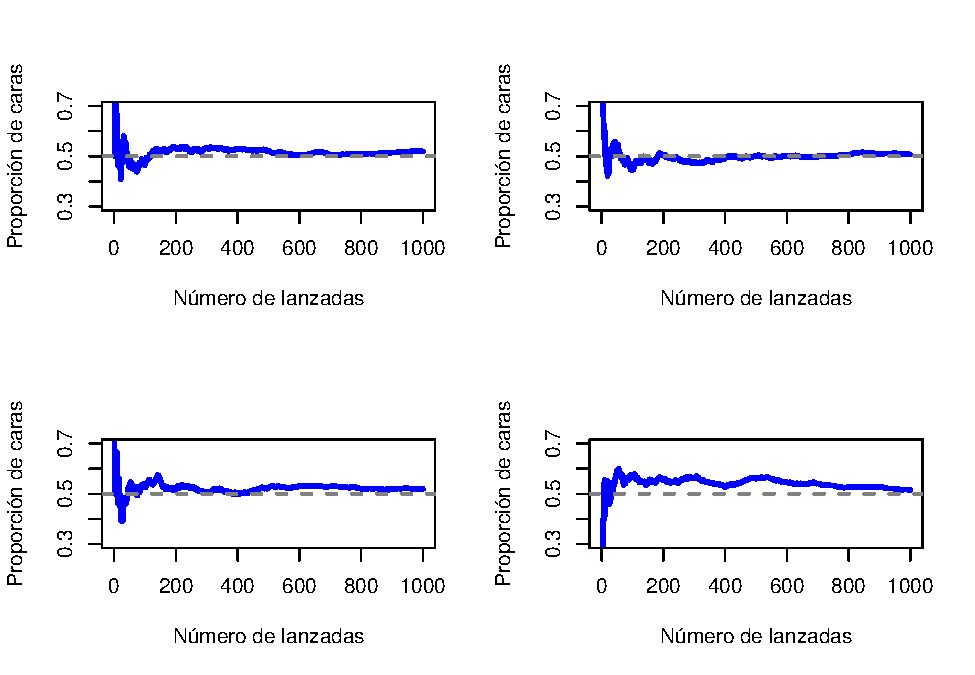
\includegraphics{FdI2_files/figure-latex/frequentistprobability-1.pdf}
\caption{\label{fig:frequentistprobability} Una imagen de cómo funciona la
probabilidad frecuentista. Si lanzas una moneda justa una y otra vez, la
proporción de caras deja de fluctuar y converge hacia la probabilidad
real de 0.5. Cada panel muestra uno de las cuatro simulaciones con 1.000
lanzamientos cada uno. Aunque ninguna de estas simulaciones terminó con
un valor exacto de .5, si hubiéramos extendido el experimento por un
número infinito de lanzamientos lo habríamos conseguido.}
\end{figure}

La definición frecuentista de probabilidad tiene algunas características
que le hacen deseable. En primer lugar, es objetivo: la probabilidad de
un evento se basa \emph{necesariamente} en el mundo real. La única forma
en que declaraciones de probabilidad puedan tener sentido es si se
refieren a (una secuencia de) eventos que ocurren en el universo físico.
En segundo lugar, es inequívoco: dos personas que miran como se
desarrolla la misma secuencia de eventos, al tratar de calcular la
probabilidad de un evento, inevitablemente deberán llegar a la misma
respuesta. Sin embargo, también tiene algunas características no tan
deseables. En primer lugar, no existen secuencias infinitas en el mundo
físico. Supongamos que has encontrado una moneda en el suelo y has
comenzado a lanzarla varias veces. Cada vez que aterriza, impacta en el
suelo. Cada impacto daña un poco la moneda; eventualmente, la moneda
será inutilizable. Entonces, uno podría preguntarse si realmente tiene
sentido fingir que una secuencia ``infinita'' de lanzamientos de monedas
es un concepto significativo u objetivo. No podemos decir que una
``secuencia infinita'' de eventos es algo real en el universo físico,
porque el universo físico no permite nada infinito. Así, podemos ver que
la definición frecuentista tiene un alcance limitado. Hay muchas cosas
por ahí a las que los seres humanos estamos felices de asignar
probabilidades en el día a día, pero que no pueden (ni siquiera en
teoría) ser planteadas como una secuencia hipotética de eventos. Por
ejemplo, si un meteorólogo aparece en televisión y dice: ``la
probabilidad de lluvia en Pamplona el 2 de noviembre del 2048 es del
60\%'' nosotros podemos aceptarlo sin rechistar. Pero desde un punto de
vista frecuentista, no queda tan claro cómo podemos definirlo. Sólo hay
una ciudad de Pamplona (en Navarra), y sólo un 2 de noviembre del 2048.
Aquí no hay una secuencia infinita de eventos, solo una cosa de una vez.
La probabilidad frecuentista nos \emph{prohíbe} hacer declaraciones de
probabilidad sobre un solo evento. Desde la perspectiva frecuentista,
lloverá mañana o o no lloverá; no hay una ``probabilidad'' que se pueda
adjuntar a un sólo evento no repetible. Sin embargo, existen algunos
trucos que los frecuentistas pueden utilizar para solucionar esta
situación. Una posibilidad es que el meteorólogo en realidad nos quiera
decir algo así: ``Existe una categoría de días para la que predigo un
60\% probabilidad de lluvia; si miramos sólo esos días para los que hago
esta predicción, entonces en el 60\% de esos días lloverá realmente''.
Es un poco extraño y contradictorio pensarlo de esta manera, pero los
frecuentistas hacen esto a veces.

\subsection{La visión bayesiana}\label{la-vision-bayesiana}

La alternativa a la visión frecuentista, la \textbf{\emph{visión
bayesiana}} de la probabilidad, a menudo se denomina visión
subjetivista, y es una visión relativamente minoritaria entre los
estadísticos, aunque ha ido ganando terreno constantemente a lo largo de
las últimas décadas. Hay muchos formas de bayesianismo, lo que hace
difícil decir exactamente cuál es ``la'' visión bayesiana. La forma más
fácil de entender la probabilidad subjetiva es al definir la
probabilidad de un evento como el \textbf{\emph{grado de creencia}} que
un agente inteligente y racional asigna a la verdad de ese evento. Desde
esa perspectiva, las probabilidades no existen en el mundo, sino más
bien en los pensamientos y suposiciones de las personas y otros seres
inteligentes. Sin embargo, para que este enfoque funcione, necesitamos
una forma de operacionalizar este ``grado de creencia''. Una forma de
hacerlo es formalizándolo en términos de una ``apuesta racional'' aunque
existen muchas otras formas. Supongamos que creo que existe una
probabilidad de que llueva mañana de un 60\%. Si alguien me hace una
apuesta, si llueve mañana, gano \$5, pero si no llueve, pierdo \$5.
Claramente, desde mi punto de vista, esta es una buena apuesta. Por otro
lado, si creo que la probabilidad de lluvia es sólo del 40\%, entonces
es una mala apuesta. Por lo tanto, podemos poner en práctica la noción
de una ``probabilidad subjetiva'' en términos de qué apuestas que estoy
dispuesto a aceptar.

¿Cuáles son las ventajas y desventajas del enfoque bayesiano? La
principal ventaja es que le permite asignar probabilidades a cualquier
evento. No esta limitado a aquellos eventos que son repetibles. La
principal desventaja (para muchas personas) es que no podemos ser
realmente objetivos - especificar una probabilidad requiere que
especifiquemos la entidad que tiene el grado de creencia que estamos
examinando. Esta entidad puede ser un humano, un extraterrestre, un
robot o incluso un estadístico, pero tiene que ser un agente inteligente
que sea capaz de creer en cosas. Para muchas personas esto representa un
inconveniente: parece hacer que la probabilidad sea arbitraria. Si bien
el enfoque bayesiano requiere que el agente en cuestión sea racional (es
decir, que obedezca las reglas de la probabilidad), permite que todos
tengan sus propias creencias; yo puedo creer que la moneda es justa
mientras que otro no, aunque ambos seamos racionales. La visión
frecuentista no permite que dos observadores atribuyan diferentes
probabilidades al mismo evento: cuando eso sucede, al menos uno de ellos
debe estar equivocado. La visión bayesiana no evita que esto ocurra. Dos
observadores con diferentes conocimientos previos pueden tener creencias
diferentes sobre el mismo evento. En otras palabras, mientras que la
visión frecuentista se puede considerar como demasiado estrecha (prohíbe
muchas cosas a las cuales queremos asignar probabilidades), la visión
bayesiana puede resultar demasiado amplia (permite demasiadas
diferencias entre observadores).

\subsection{¿Cuál es la diferencia? ¿Y quién tiene
razón?}\label{cual-es-la-diferencia-y-quien-tiene-razon}

Ahora que hemos visto ambas visiones estadísticas de forma
independiente, es necesario compararlas. Regresemos al hipotético juego
de fútbol de robots que comentamos comienzo del tema. ¿Que dirían un
frecuentista y un bayesiano sobre las tres afirmaciones? ¿Qué enunciado
sería la definición de probabilidad correcta para el frecuentista? ¿Y
para el bayesiano? ¿Es posible que alguno de los enunciados no tenga
sentido para cualquiera de los dos? Si entendemos ambas perspectivas,
podemos intuir cómo responder a estas preguntas.

Entendiendo las diferencias, podemos preguntarnos a continuación cuál de
dos enfoques es el \emph{correcto}. Sin embargo, no existe una respuesta
correcta. Matemáticamente hablando, no hay nada incorrecto sobre la
forma en que los frecuentistas piensan sobre secuencias de eventos, ni
hay nada incorrecto acerca de la forma en que los bayesianos definen las
creencias de un agente racional. De hecho, si vamos al detalle, los
bayesianos y los frecuentistas en realidad están de acuerdo en muchas
cosas. Muchos métodos frecuentistas conducen a decisiones que los
bayesianos pensarían que toma un agente racional. Muchos métodos
bayesianos tienen buenas propiedades frecuentistas.

En cualquier caso, la mayor parte de los métodos y análisis estadísticos
en la literatura se basan en el enfoque frecuentista. Por lo tanto, el
objetivo de esta asignatura es cubrir aproximadamente el mismo temario
que una clase típica de estadística de pregrado en ciencias de la
educación, y si queremos entender las herramientas estadísticas
utilizadas por la mayoría de los educadores en investigación,
necesitaremos una buena comprensión de los métodos frecuentistas.

\section{Teoría de probabilidad básica}\label{basicprobability}

A pesar de los argumentos ideológicos entre bayesianos y frecuentistas,
existe un consenso más o menos generalizado sobre las reglas que la
probabilidad debe obedecer. Hay muchas formas de abordar estas reglas.
El enfoque más utilizado se basa en el trabajo de Andrey Kolmogorov, uno
de los grandes matemáticos soviéticos del siglo XX. No entraremos mucho
en detalle, pero aprenderemos en qué consisten y cómo utilizarlas a
través del siguiente ejemplo.

\subsection{Introducción a las distribuciones de
probabilidad}\label{introduccion-a-las-distribuciones-de-probabilidad}

Un hecho comprobado sobre mi vida es que sólo tengo 5 pares de
pantalones: tres pares de vaqueros, los pantalones de un traje y un par
de pantalones de chándal. Lo más triste es que les he dado nombres: los
llamo \(X_1\), \(X_2\), \(X_3\), \(X_4\) y \(X_5\). Diariamente, por la
mañana, elijo un único par de esos pantalones que voy a usar. Si yo
tuviera que describir esta situación usando el lenguaje de la teoría de
la probabilidad, me referiría a cada par de pantalones (es decir, a cada
\(X\)) como un \textbf{\emph{evento elemental}}. La característica clave
de estos eventos elementales es que cada vez que hacemos una observación
(por ejemplo, cada vez que escojo un par de pantalones), el resultado
será uno y solo uno de estos eventos. Como he dicho antes, siempre uso
exactamente sólo un par de pantalones, así que mis pantalones cumplen
con esta restricción. Del mismo modo, al conjunto de todos los eventos
posibles se le denomina \textbf{\emph{espacio muestral}}. Siguiendo con
el ejemplo, mi espacio muestral sería el armario que contiene los 5
pantalones.

Bien, ahora que tenemos un espacio muestral (un armario), que está
construido a partir de muchas posibles eventos elementales (pantalones),
lo que queremos hacer es asignar una \textbf{\emph{probabilidad}} a cada
uno de estos eventos elementales. Para un evento \(X\), la probabilidad
de ese evento \(P(X)\) es un número que se encuentra entre 0 y 1. Cuanto
mayor sea el valor de \(P(X)\), más probable será que ocurra el evento.
Entonces, por ejemplo, si \(P(X) = 0\), significa que el evento \(X\) es
imposible (es decir, nunca uso esos pantalones). Por otro lado, si
\(P(X) = 1\) significa que el evento \(X\) es seguro que ocurra (es
decir, siempre uso esos pantalones). Los valores de probabilidad
intermedios, significan que a veces uso esos pantalones (y a veces no).
Por ejemplo, una \(P(X) = 0.5\) significa que uso esos pantalones la
mitad de las veces.

Llegados a este punto, lo siguiente que debemos entender es que ``algo
siempre sucede''. Cada vez que me pongo unos pantalones, realmente
termino usando esos pantalones. Lo que esto significa en términos
probabilísticos, es que las probabilidades de todos los eventos
elementales siempre suman 1. Esto se conoce como la \textbf{\emph{ley de
probabilidad total}}. Si se cumplen estos requisitos (tenemos número
\(X\) de pantalones, cada par con una probabilidad \(P(X)\) de usarlos
que en total suman 1), entonces lo que tenemos es una
\textbf{\emph{distribución de probabilidad}}.Veamos un ejemplo de
distribución de probabilidad

\begin{longtable}[]{@{}llllll@{}}
\toprule
Pantalones & V..azules & V..grises & V..negros & Traje.negro &
Chándal.azul\tabularnewline
\midrule
\endhead
Nombre & \(X_1\) & \(X_2\) & \(X_3\) & \(X_4\) & \(X_5\)\tabularnewline
Probabilidad & \(P(X_1) = .5\) & \(P(X_2) = .3\) & \(P(X_3) = .1\) &
\(P(X_4) = 0\) & \(P(X_5) = .1\)\tabularnewline
\bottomrule
\end{longtable}

Cada uno de estos eventos tiene una probabilidad que se encuentra entre
0 y 1, y si sumamos la probabilidad de todos eventos, suman 1. Incluso
podemos dibujar un gráfico de barras para visualizar esta distribución,
como se muestra en la Figura \ref{fig:pantsprob}.

\begin{figure}
\centering
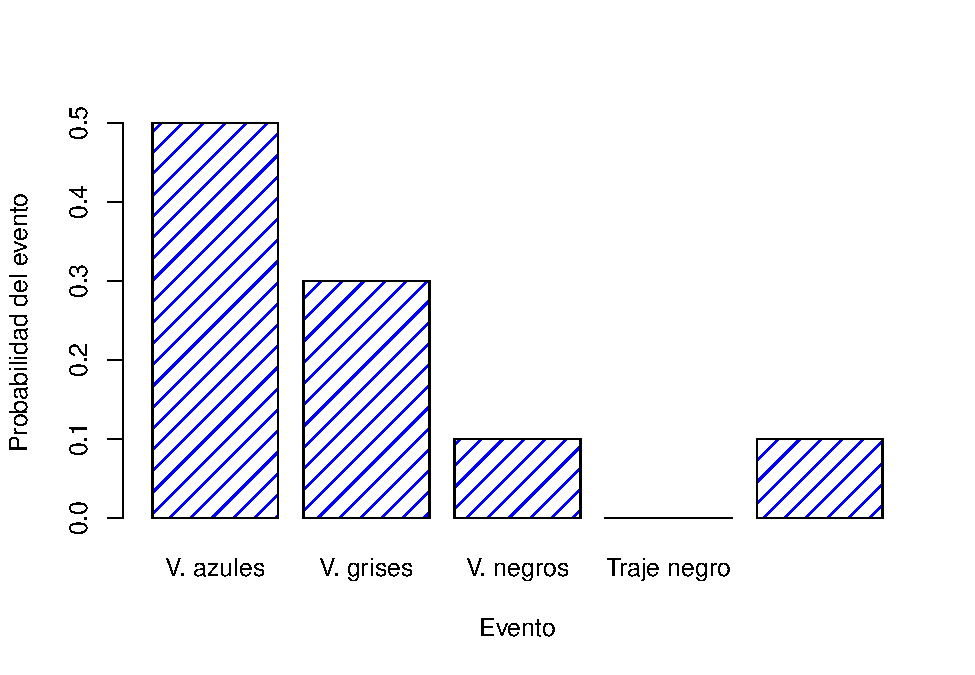
\includegraphics{FdI2_files/figure-latex/pantsprob-1.pdf}
\caption{\label{fig:pantsprob}Demostración visual de la distribución de
probabilidad de los ``pantalones''. Existen 5 ``eventos elementales'',
que se corresponden con mis 5 pares de pantalones. Cada evento tiene una
probabilidad de ocurrir: esta probabilidad es un número entre 0 y 1. La
suma de estas probabilidades es 1.}
\end{figure}

Es importante señalar que la teoría de probabilidades permite hablar
acerca de eventos elementales pero también sobre los
\textbf{\emph{eventos no elementales}}. La forma más fácil de ilustrar
este concepto es con un ejemplo. Siguiendo con el ejemplo de los
pantalones, es perfectamente posible hablar sobre la probabilidad de
usar vaqueros. Bajo esta premisa, podemos decir que el evento ``yo uso
vaqueros'' es posible siempre y cuando ocurra alguno de los eventos
elementales apropiados; en este caso ``vaqueros azules'', ``vaqueros
negros'' o ``vaqueros grises''. En términos matemáticos, definimos al
evento \(E\) ``vaqueros'' como el conjunto de eventos elementales
\((X_1, X_2, X_3)\). Si se produce alguno de estos eventos elementales,
también podemos decir que \(E\) ha ocurrido. Por lo tanto, podemos decir
que la probabilidad \(P(E)\) es simplemente la suma de esos tres
eventos, así \[
P(E) = P(X_1) + P(X_2) + P(X_3)
\] y, dado que las probabilidades de los vaqueros azules, grises y
negros son respectivamente .5, .3 y .1, la probabilidad total de usar
vaqueros es igual a .9.

Todo esto parece obvio y simple. Sin embargo, a partir de estos simples
comienzos, es posible construir algunas herramientas matemáticas más
complejas y poderosas. En la siguiente Tabla se muestran algunas de las
otras reglas que deben de cumplirse para poder calcular probabilidades.

\begin{longtable}[]{@{}llll@{}}
\toprule
Castellano & Notacion & Igual & Formula\tabularnewline
\midrule
\endhead
No \(A\) & \(P(\neg A)\) & = & \(1-P(A)\)\tabularnewline
\(A\) o \(B\) & \(P(A \cup B)\) & = &
\(P(A) + P(B) - P(A \cap B)\)\tabularnewline
\(A\) y \(B\) & \(P(A \cap B)\) & = &
\(P(A \vert B) P(B)\)\tabularnewline
\bottomrule
\end{longtable}

\section{La distribución binomial}\label{binomial}

Como hemos visto, las distribuciones de probabilidad pueden variar
enormemente, por lo que existe un gran número de distribuciones
posibles. Sin embargo, no todas son igual de importantes. Las
distribuciones más importantes, y de las que hablaremos en esta
asignatura son cinco: la distribución binomial, la distribución normal,
la distribución \(t\), la distribución \(\chi^2\) (``chi-cuadrada'') y
la distribución \(F\). Daremos una breve introducción a las cinco,
prestando especial atención a las distribuciones binomial y normal.
Comenzaremos con la distribución más simple de las cinco, la
distribución binomial.

\subsection{Introducción al binomio}\label{introduccion-al-binomio}

La teoría de la probabilidad se creó originalmente para intentar
describir cómo funcionaban los juegos de azar, por lo que parece
adecuado que nuestra discusión sobre la \textbf{\emph{distribución
binomial}} involucre una discusión sobre tirar dados y lanzar monedas.
Imaginemos el siguiente ``experimento'': tengo en mi poder 20 dados
iguales de seis caras. En una de las caras de cada dado hay una imagen
de una calavera; las otras cinco caras están en blanco. Si tiro los 20
dados, ¿cuál es la probabilidad de que obtenga exactamente 4 calaveras?
Asumiendo que los dados son justos, sabemos que la probabilidad de que
en un dado salga la calavera es de de 1 en 6; dicho de otra forma, la
probabilidad de que salga calavera en un solo dado es de aproximadamente
\(.167\). Esta información es suficiente para poder responder a nuestra
pregunta anterior, así que veamos cómo hacerlo.

Primero, pondremos algunos nombres a los eventos con su respectiva
notación. Dejaremos que \(N\) denote el número de dados que se tiran en
nuestro experimento; a esto se le conoce como el \textbf{\emph{parámetro
de tamaño}} de nuestra distribución binomial. También usaremos
\(\theta\) para referirnos a la probabilidad de que al tirar un solo
dado salga calavera, una cantidad que generalmente se denomina como la
\textbf{\emph{probabilidad de éxito}} del binomio.\footnote{Hay que
  tener en cuenta que el término ``éxito'' es bastante arbitrario, y en
  realidad no implica que el resultado sea algo deseado. Si \(\theta\)
  se refiriera a la probabilidad de que un pasajero se lesione en un
  accidente de autobús, seguiría siendo una probabilidad de éxito,
  aunque en realidad no queremos que la gente salga lastimada}
Finalmente, usaremos \(X\) para referirnos a los resultados de nuestro
experimento, es decir, la cantidad de calaveras que obtengo cuando lanzo
los dados. Dado que el valor real de \(X\) se debe al azar, nos podemos
referir a ella como una \textbf{\emph{variable aleatoria}}. En cualquier
caso, ahora que tenemos toda esta terminología y notación, podemos
utilizarlos para exponer el problema que planteábamos en el párrafo
anterior con mayor precisión. La cantidad que queremos calcular es la
probabilidad de que \(X = 4\) sabiendo que \(\theta = .167\) y \(N=20\).
La ``forma'' general de esta probabilidad que me interesa calcular
podría escribirse como, \[
  P(X \ | \ \theta, N)
\] donde estamos interesados en el caso específico donde \(X=4\),
\(\theta = .167\) y \(N=20\). Hace falta un elemento de notación más
antes de continuar con la solución del problema. Si yo quiero decir que
\(X\) se genera aleatoriamente a partir de una distribución binomial con
los parámetros \(\theta\) y \(N\), la notación que usaría para
expresarlo sería la siguiente: \[
  X \sim \mbox{Binomial}(\theta, N)
\]

Aunque no utilizaremos las fórmulas para hacer cálculos formalmente,
dejaré la fórmula de la distribución binomial en la Tabla
\ref{tab:distformulas}, ya que puede ser útil si se quieren entender
temas más avanzados con algo de profundidad. Por lo pronto, analizaremos
como se ve una distribución binomial (puedes hacerlo tú mismo si entras
\href{https://leudave.shinyapps.io/distribuciones/}{aquí}). La Figura
\ref{fig:binomial1} dibuja la probabilidad binomial para todos los
valores posibles de \(X\) de nuestro experimento de lanzamiento de
dados, partiendo desde \(X=0\) (ninguna sale calavera) hasta \(X=20\)
(salen todas calaveras). Hay que tener en cuenta que esto es básicamente
un gráfico de barras, al igual que la gráfica de la ``probabilidad de
pantalones'' de la Figura \ref{fig:pantsprob}. En el eje horizontal
tenemos todos los eventos posibles, y en el eje vertical podemos leer la
probabilidad de que ocurra cada uno de esos eventos. Por lo tanto, la
probabilidad de que salgan 4 calaveras al tirar 20 dados es de
aproximadamente 0,20 (la respuesta exacta es 0,2022036, como veremos en
un momento). En otras palabras, esperaría que ese evento suceda
aproximadamente el 20\% de las veces que se lleve a cabo este
experimento.

\begin{table}[t]

\caption{\label{tab:distformulas}Fórmulas para las distribuciones binomial y normal. En la ecuación de la binomial, $X!$ es una función factorial (es decir, multiplica todos los números enteros de  1 hasta $X$), y en la de la distribución normal "exp" se refiere a una función exponencial.}
\centering
\begin{tabular}{l|l}
\hline
Binomial & Normal\\
\hline
\$P(X | \textbackslash{}theta, N) = \textbackslash{}displaystyle\textbackslash{}frac\{N!\}\{X! (N-X)!\}  \textbackslash{}theta\textasciicircum{}X (1-\textbackslash{}theta)\textasciicircum{}\{N-X\}\$ & \$p(X | \textbackslash{}mu, \textbackslash{}sigma) = \textbackslash{}displaystyle\textbackslash{}frac\{1\}\{\textbackslash{}sqrt\{2\textbackslash{}pi\}\textbackslash{}sigma\} \textbackslash{}exp \textbackslash{}left( -\textbackslash{}frac\{(X - \textbackslash{}mu)\textasciicircum{}2\}\{2\textbackslash{}sigma\textasciicircum{}2\} \textbackslash{}right)\$\\
\hline
\end{tabular}
\end{table}

\begin{figure}
\centering
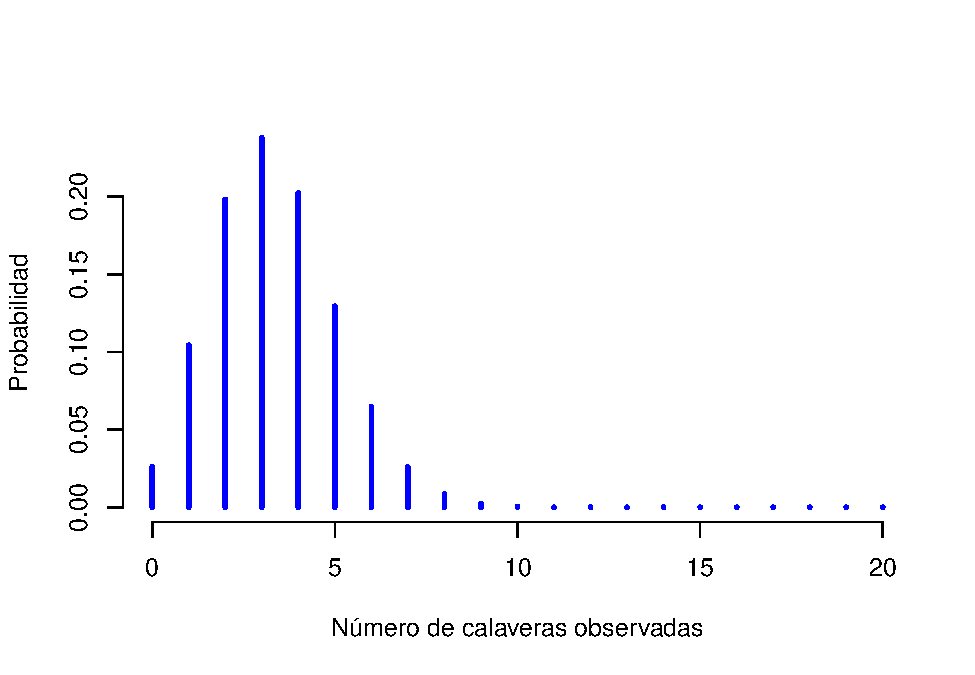
\includegraphics{FdI2_files/figure-latex/binomial1-1.pdf}
\caption{\label{fig:binomial1} La distribución binomial con parámetro de
tamaño de \(N=20\) y una probabilidad de éxito de \(theta = 1/6\). Cada
barra vertical representa la probabilidad de un resultado específico (un
valor posible de \(X\)). Ya que esta es una distribución de
probabilidad, cada una de las probabilidades debe ser un número entre 0
y 1, y la altura de las barras también deben sumar 1.}
\end{figure}

Para darte una idea de cómo cambia la distribución binomial cuando
modificamos los valores de \(\theta\) y \(N\), supongamos que en lugar
de tirar dados, en realidad estoy lanzando monedas. Esta vez, mi
experimento implica lanzar una moneda justa repetidamente, y el
resultado que me interesa es la cantidad de caras que observo. En este
escenario, la probabilidad de éxito ahora es de \(\theta = 1/2\).
Supongamos que tirara la moneda \(N=20\) veces. En este ejemplo, he
cambiado la probabilidad de éxito, pero mantuve el tamaño de la muestra
del experimento. ¿Qué efecto tiene este cambio en nuestra distribución
binomial? Bueno, como la Figura \ref{fig:binomial2a} muestra, el efecto
principal fue el desplazamiento de toda la distribución hacia la
derecha, como era de esperar. ¿Y si lanzamos una moneda \(N=100\) veces?
En este caso obtendremos algo como lo de la Figura \ref{fig:binomial2b}.
La distribución se mantiene aproximadamente en el medio, pero hay un
poco más de variabilidad en los posibles resultados.

\begin{figure}
\centering
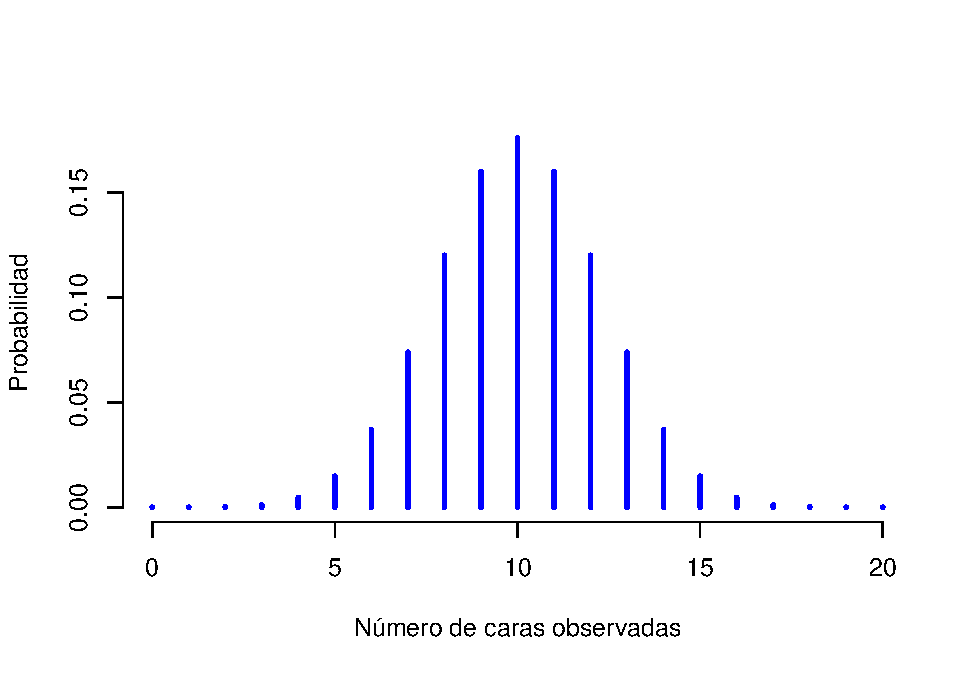
\includegraphics{FdI2_files/figure-latex/binomial2a-1.pdf}
\caption{\label{fig:binomial2a}Dos distribuciones binomiales, que involucran
un escenario en el que lanzo una moneda justa, donde la probabilidad de
éxito es \(theta = 1/2\). Asumimos que estoy lanzando la moneda \(N=20\)
veces.}
\end{figure}

\begin{figure}
\centering
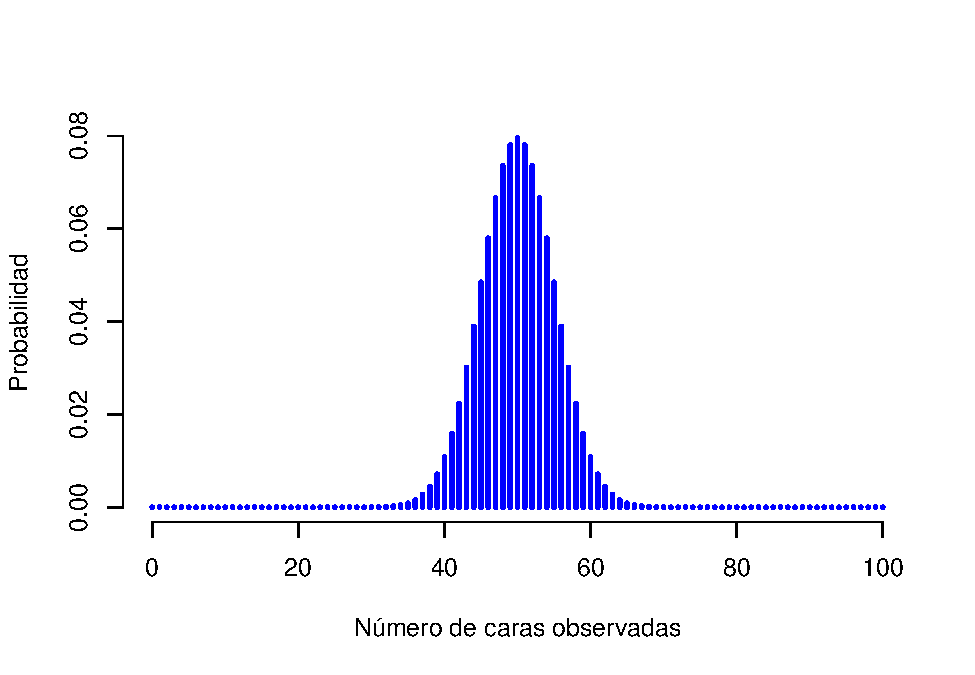
\includegraphics{FdI2_files/figure-latex/binomial2b-1.pdf}
\caption{\label{fig:binomial2b}Dos distribuciones binomiales, que involucran
un escenario en el lanzo una moneda justa, donde la probabilidad de
éxito subyacente es \(theta = 1/2\). Asumimos que estoy lanzando la
moneda \(N=100\) veces.}
\end{figure}

\section{La distribución normal}\label{normal}

Si bien la distribución binomial es conceptualmente la distribución más
sencilla de entender, no es la más importante. Ese honor le corresponde
a la \textbf{\emph{distribución normal}}, también conocida como ``curva
de campana'' o como ``distribución gaussiana'' o ``campana de Gauss''.
Una distribución normal se describe utilizando dos parámetros, la media
de la distribución \(\mu\) y la desviación estándar de la distribución
\(\sigma\). La notación que utilizamos para decir que una variable \(X\)
se distribuye normalmente es la siguiente:

\[
  X \sim \mbox{Normal}(\mu,\sigma)
\] Al igual que con la distribución binomial, he incluido la fórmula
para la distribución normal en la tabla \ref{tab:distformulas}, porque
creo que es lo suficientemente importante como para que todos los que
aprenden algo de estadística al menos la conozcan, aunque no nos
enfoquemos en ella.

Vamos intentar descifrar lo que significa que una variable esté
normalmente distribuida. Echemos un vistazo a la Figura
\ref{fig:normdist}, que muestra una distribución normal con media
\(\mu = 0\) y desviación estándar \(\sigma = 1\). Con un poco de
imaginación, podemos apreciar de dónde viene el nombre ``curva de
campana''. A diferencia de los gráficos sobre la distribución binomial,
la imagen de la distribución normal en la Figura \ref{fig:normdist}
muestra una curva suave en lugar de barras ``tipo histograma''. Esto no
es arbitrario: la distribución normal es continua, mientras que la
distribución binomial es discreta. Por ejemplo, en el experimento de
tiro de dados de la sección anterior, es posible obtener 3 calaveras o 4
calaveras, mientras que un valor intermedio como 3.9 es imposible de
obtener. Este hecho se ve reflejado en la Figura \ref{fig:binomial1},
donde tenemos una barra ubicada en \(X=3\) y otra en \(X=4\), pero entre
ellas no hay nada. En cambio, los valores continuos no tienen esta
restricción. Por ejemplo, supongamos que estamos hablando del tiempo. La
temperatura de un día primavera podría ser de 23 grados, 24 grados, 23.9
grados o cualquier cosa intermedia, ya que la temperatura es una
variable continua, por lo que una distribución normal podría ser la
herramienta apropiada para describir las diferentes temperaturas en los
días de primavera.\footnote{En la práctica, la distribución normal es
  tan útil que las personas tienden a usarla incluso cuando la variable
  no es continua. Siempre que haya suficientes categorías (por ejemplo,
  respuestas de escala Likert de un cuestionario), suele ser frecuente
  el uso de la distribución normal.}

\begin{figure}
\centering
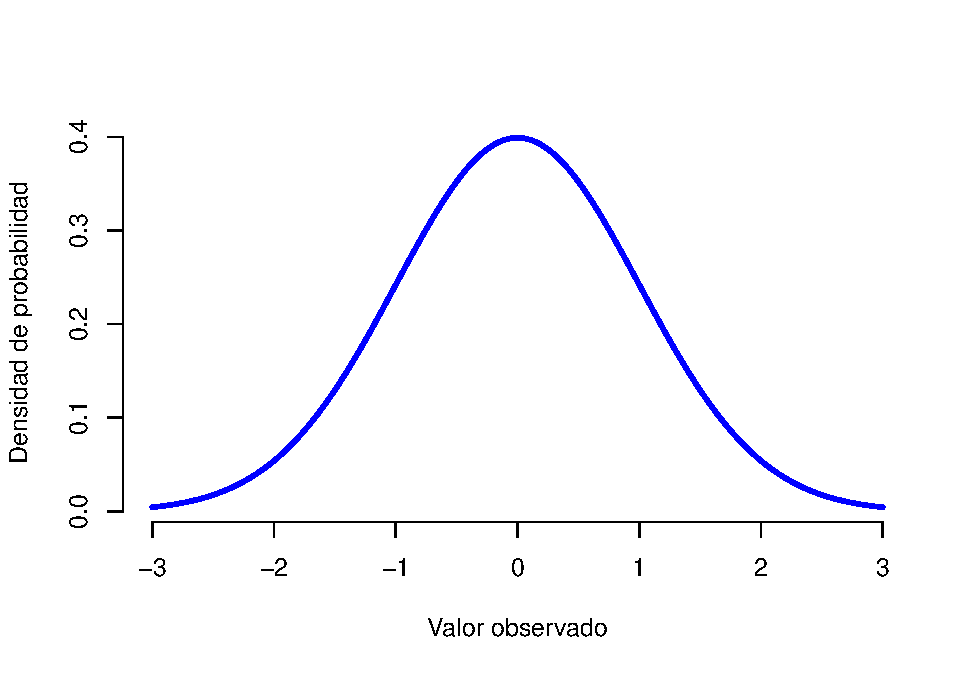
\includegraphics{FdI2_files/figure-latex/normdist-1.pdf}
\caption{\label{fig:normdist} Distribución normal con media \(mu = 0\) y
desviación estándar \(sigma = 1\). El eje \(x\) corresponde con el valor
de alguna variable, y el eje \(y\) nos dice qué tan probable es que
observemos ese valor. Sin embargo, vemos como el eje \(y\) se denomina
``Densidad de Probabilidad'' y no ``Probabilidad''. La altura de la
curva no representa como tal la probabilidad de observar un valor
particular de \(x\). Sin embargo, las alturas nos informan sobre qué
valores de \(x\) son más probables (¡los más altos!).}
\end{figure}

Una vez visto esto, vamos a analizar cómo funciona una distribución
normal. En primer lugar, veamos qué es lo que sucede cuando jugamos con
los parámetros de la distribución (puedes hacerlo tú mismo si entras en
este enlace). La Figura \ref{fig:normmean} muestra distribuciones
normales que tienen medias diferentes, pero con la misma desviación
estándar. Como es de esperar, todas estas distribuciones tienen la misma
``anchura''. La unica diferencia entre ellas es que se han desplazado
hacia la izquierda o hacia la derecha. En todos los demás aspectos son
idénticas. Por el contrario, si aumentamos la desviación estándar
mientras mantenemos la media constante, el pico de la distribución
permanece en el mismo lugar, pero la distribución se amplía, como
podemos ver en la Figura \ref{fig:normsd}. Sin embargo, cuando ampliamos
la distribución, la altura del pico disminuye. Esto \emph{tiene} que
suceder: de la misma forma que las alturas de las barras de una
distribución binomial discreta tienen que \emph{sumar} 1, el total del
\emph{área bajo la curva} de una distribución normal debe ser igual a 1.

\begin{figure}
\centering
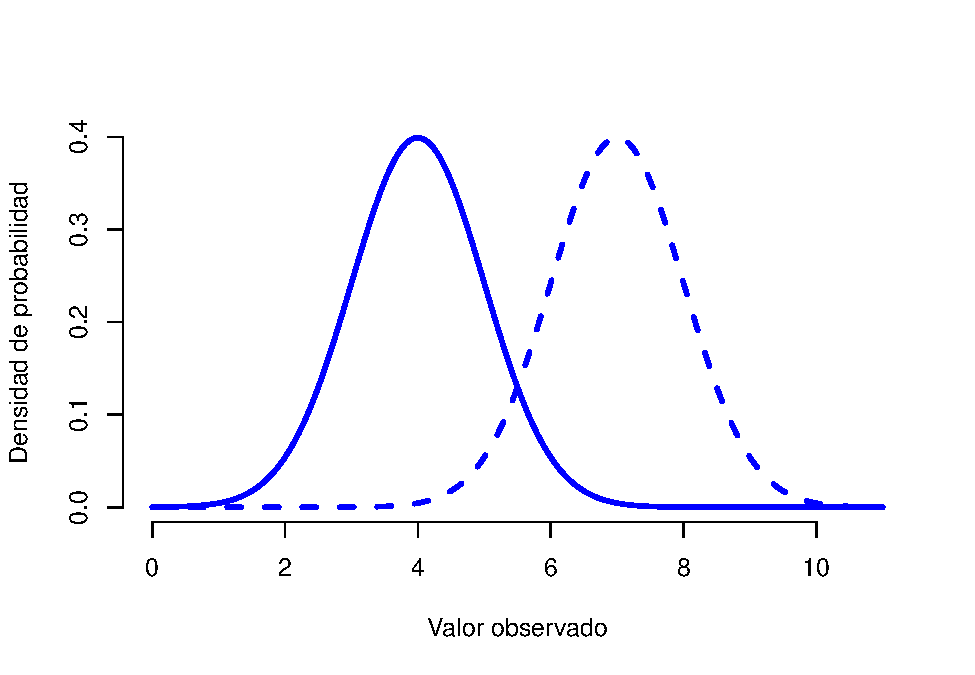
\includegraphics{FdI2_files/figure-latex/normmean-1.pdf}
\caption{\label{fig:normmean}Gráfica que demuestra lo que sucede cuando se
cambia la media de una distribución normal. La línea sólida representa
una distribución normal con media de \(mu=4\). La línea discontinua
muestra una distribución normal con una media de \(mu=7\). En ambos
casos, la desviación estándar es de \(sigma=1\). Vemos como las dos
distribuciones tienen la misma forma, pero la distribución con la línea
discontinua se desplaza hacia la derecha.}
\end{figure}

\begin{figure}
\centering
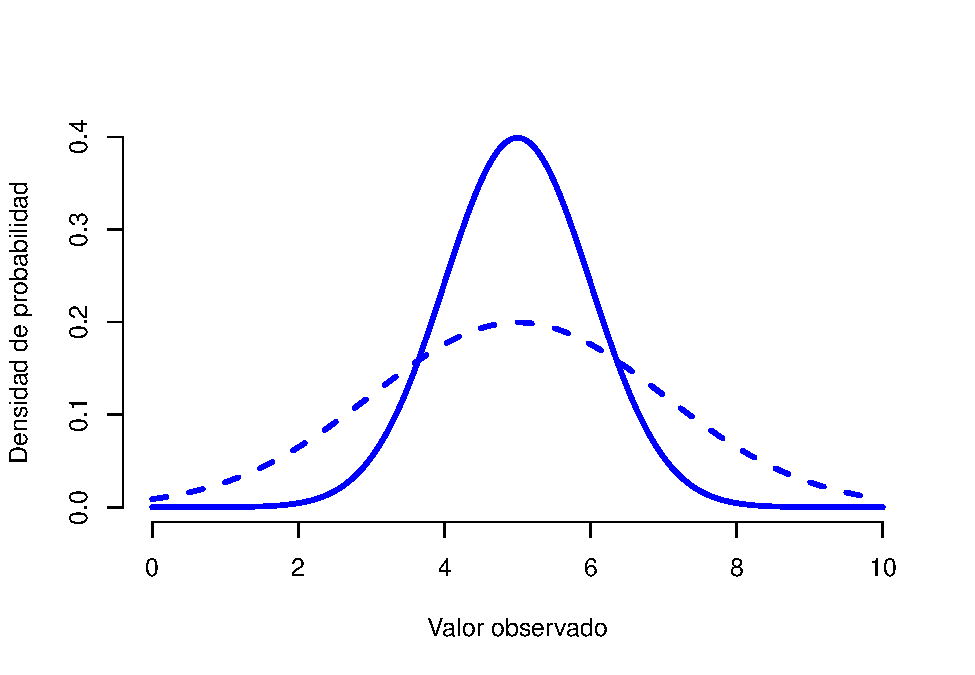
\includegraphics{FdI2_files/figure-latex/normsd-1.pdf}
\caption{\label{fig:normsd}Una ilustración de lo que sucede cuando cambia la
desviación estándar de una distribución normal. Ambas distribuciones
tienen una media de \(mu=5\), pero diferentes desviaciones estándar. La
línea continua dibuja una distribución con una desviación estándar
\(sigma=1\), y la línea discontinua muestra una distribución con
desviación estándar de \(sigma=2\). Como consecuencia, ambas
distribuciones están centradas en el mismo lugar, pero la distribución
con la línea discontinua es más ancha que la otra.}
\end{figure}

Antes de seguir adelante, quiero señalar una característica importante
de la distribución normal. Independientemente de los valores de la media
y la desviación estándar, un 68.3\% del área de la curva cae dentro de 1
desviación estándar sobre la media. Del mismo modo, el 95.4\% de la
distribución cae dentro de 2 desviaciones estándar sobre la media, y el
99.7\% de la distribución está dentro de 3 desviaciones estándar. Esta
idea se ilustra en las Figuras \ref{fig:sdnorm1} y \ref{fig:sdnorm2}.

\begin{figure}
\centering
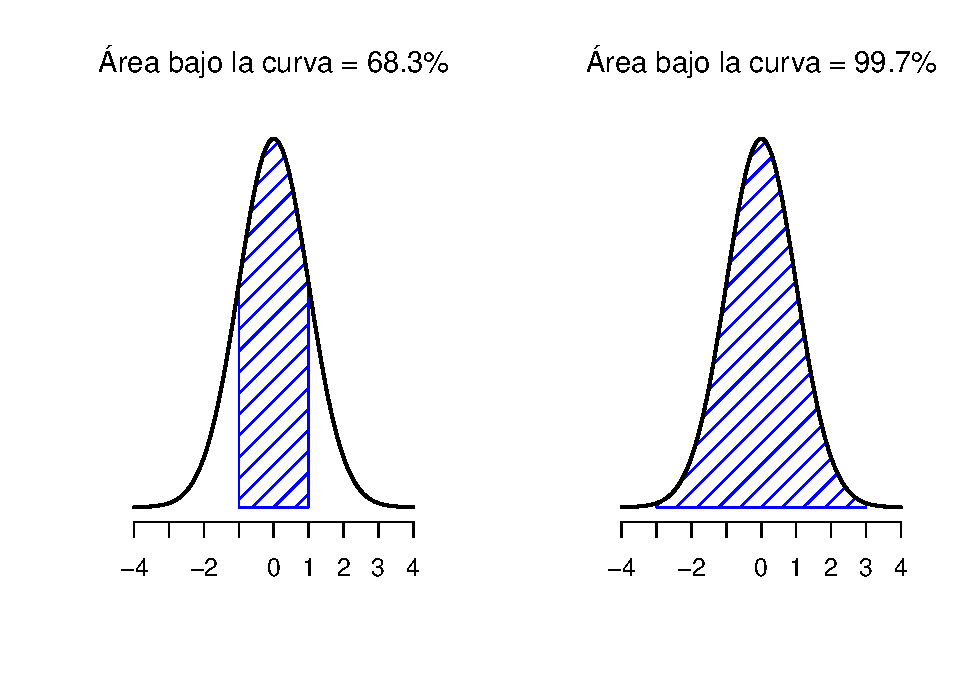
\includegraphics{FdI2_files/figure-latex/sdnorm1-1.pdf}
\caption{\label{fig:sdnorm1}El área bajo la curva indica la probabilidad de
que una observación se encuentre dentro de un rango determinado. Las
línea continua traza una distribución normal con media \(mu=0\) y
desviación estándar \(sigma=1\). El área sombreada ilustra el `área bajo
la curva' para dos casos importantes. En el panel a, podemos ver que hay
es un 68.3\% de probabilidad de que una observación caiga dentro de 1
desviación estándar sobre la media. En el panel b, vemos que existe una
probabilidad del 95.4\% de que una observación se encuentre dentro de 2
desviaciones estándar sobre la media.}
\end{figure}

\begin{figure}
\centering
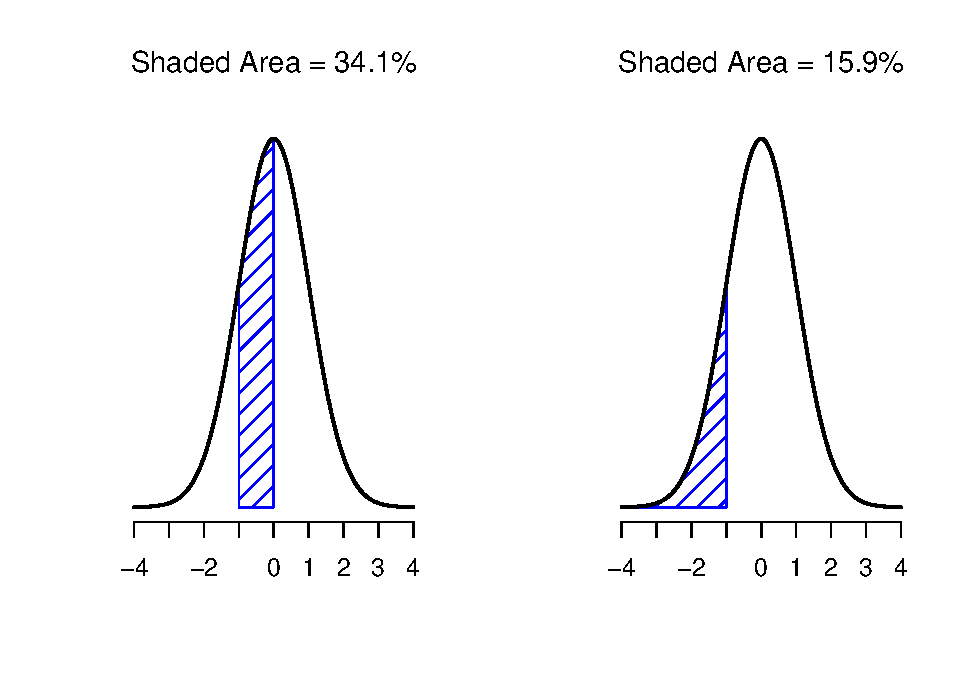
\includegraphics{FdI2_files/figure-latex/sdnorm2-1.pdf}
\caption{\label{fig:sdnorm2}Dos ejemplos más sobre el concepto del `área
bajo la curva'. Existe un 15.9\% de probabilidad de que una observación
se encuentre 1 desviación estándar o menos por debajo de la media (panel
a), y una probabilidad del 34.1\% de que una observación sea mayor que
una desviación estándar por debajo de la media pero menor que la media
(panel b). Si sumamos estos dos valores, obtendremos 15.9\% + 34.1\% =
50\%. Para datos que estén normalmente distribuidos, existe un 50\% de
probabilidad de que una observación caiga por debajo de la media. Esto
implica que existe un 50\% de probabilidad de que caiga por encima de la
media.}
\end{figure}

\subsection{Densidad de probabilidad}\label{density}

A lo largo de la discusión sobre la distribución normal, ha habido un
par de cosas que parecen no tener sentido. Quizás hayas notado que el
eje \(y\) en estas Figuras se denomina como ``Densidad de probabilidad''
en lugar de ``Probabilidad''. Tal vez notaste que utilizamos \(p(X)\) en
lugar de \(P(X)\) en la fórmula de la distribución normal.

Si utilizamos la Figura y calculamos (siguiendo la fórmula) la
probabilidad de \texttt{x\ =\ 1}, para una variable normalmente
distribuida con \texttt{media\ =\ 1} y desviación estándar
\texttt{sd\ =\ 0.1}, nos arrojará como resultado una probabilidad de
3.99. Sin embargo, hemos visto anteriormente que las probabilidades
\emph{no} pueden ser mayores que 1. Entonces, ¿qué es lo que hemos
calculado?

Lo que hemos calculado aquí en realidad no es una probabilidad: Para
entender qué es ese algo, tenemos que pensar qué es lo que realmente
\emph{significa} decir que \(X\) es una variable continua. Digamos que
estamos hablando de la temperatura otra vez. El termómetro me dice que
hacen 23 grados, pero yo sé que eso no es del todo cierto. No hacen 23
grados \emph{exactamente}. Quizás sea algo más cercano a los 23.1 grados
o, si seguimos, en realidad podrían ser 23.095 grados. Esto es lo que
sucede con los valores continuos: nunca se sabe el valor exacto.

Ahora pensemos en lo que esto implica cuando hablamos de probabilidades.
Supongamos la temperatura máxima para mañana se toma de una distribución
normal con media 23 y desviación estándar 1. ¿Cuál es la probabilidad de
que la temperatura sea \emph{exactamente} 23 grados? La respuesta es
``cero'', o posiblemente, ``un número tan cercano a cero que bien podría
ser cero''. ¿Por qué es esto? Es como intentar tirar un dardo en un
tablero de dardos con dianas infinitamente cada vez más pequeñas: no
importa cuán buena sea tu puntería, nunca acertarás. En la vida real
nunca obtendremos el valor exacto de 23. Siempre será 23.1 o 22.99998 o
algo así. En en otras palabras, no tiene sentido hablar de la
probabilidad de que la temperatura sea exactamente 23 grados. Sin
embargo, en el día a día, si el termómetro indica 23 grados pero en
realidad hacen 22.9998 grados, probablemente no nos importe demasiado.
Esto es porque en el día a día, ``23 grados'' por lo general significa
algo así como ``en algún lugar entre 22.5 y 23.5 grados''. Y aunque no
parezca muy importante preguntar por la probabilidad de que la
temperatura sea exactamente 23 grados, lo que sí lo parece es preguntar
sobre la probabilidad de que la temperatura se encuentre entre 22.5 y
23.5, o entre 20 y 30, o cualquier otro rango de temperaturas en el que
estemos interesados.

El objetivo de esta explicación es dejar claro que, cuando hablamos de
distribuciones continuas, no tiene sentido hablar sobre la probabilidad
de un valor específico. Sin embargo, sí que \emph{podemos} hablar sobre
la probabilidad de que el valor se encuentre dentro de un rango
particular de valores. Para encontrar probabilidad asociada con un rango
particular, lo que debe hacer es calcular el ``área bajo la curva''.
Este concepto lo conocemos: en la Figura \ref{fig:sdnorm1}, las áreas
sombreadas representan probabilidades genuinas (por ejemplo, la Figura
\ref{fig:sdnorm1} muestra la probabilidad de observar un valor que cae
dentro de 1 desviación estándar sobre la media).

Para finalizar, volveremos con la fórmula para \(p(x)\) que vimos
anteriormente. Los resultados de \(p(x)\) no describe una probabilidad,
sino una \textbf{\emph{densidad de probabilidad}}, que en las gráficas
corresponde a la altura de la curva. De la misma forma en que las
probabilidades son números no-negativos que deben sumar 1, las
densidades de probabilidad son números no-negativos que deben integrar a
1 (donde la integral se toma a través de todos los valores posibles de
\(X\)). Para calcular la probabilidad de que \(X\) caiga entre \(a\) y
\(b\) calculamos la integral definida de la función de densidad sobre el
rango correspondiente, \(\int_a^b p(x) \ dx\). Se trata simplemente de
otra forma de llegar al mismo resultado.

\section{Otras distribuciones útiles}\label{otherdists}

La distribución normal es la distribución más utilizada por los
estadísticos (por razones que se discutirán más adelante), y la
distribución binomial es útil muchos escenarios. Sin embargo, existen
otros tipos de distribuciones de probabilidad. Revisaremos brevemente 3
de ellas: la distribución \(t\), la distribución \(\chi^2\) y la
distribución \(F\). La \textbf{\emph{distribución \(t\)}} es una
distribución continua que se parece mucho a una distribución normal,
pero que tiene colas más pesadas (ver Figura \ref{fig:tdist}). Esta
distribución tiende a surgir en situaciones en las que piensa que los
datos siguen una distribución normal, pero no se conoce la media o la
desviación estándar.

\begin{figure}
\centering
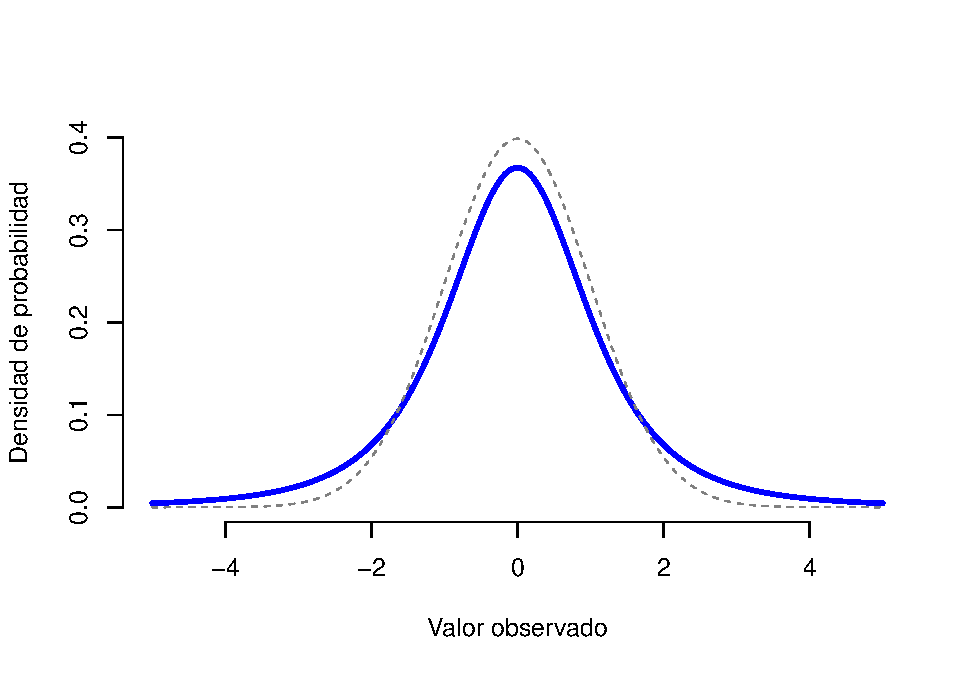
\includegraphics{FdI2_files/figure-latex/tdist-1.pdf}
\caption{\label{fig:tdist}Una distribución \(t\) con 3 grados de libertad
(línea continua). Se asemeja a una distribución normal, pero no es igual
(línea discontinua). Ten en cuenta que las ``colas'' de la distribución
\(t\) son más ``pesadas'' (es decir, se extienden más hacia afuera,
conteniendo más valores que se alejan de la media) que las colas de la
distribución normal.}
\end{figure}

\begin{itemize}
\tightlist
\item
  La \textbf{\emph{distribución \(\chi^2\)}} es otra distribución que
  podemos encontrar con cierta frecuencia. Es habitual encontrarla
  cuando hacemos análisis de datos categóricos. Los valores de una
  distribución \(\chi^2\) se consiguen al elevar al cuadrado los valores
  de una variable distribuída normalmente y luego sumarlos (un
  procedimiento denominado ``suma de cuadrados''). Después veremos
  porqué es útil hacer una ``suma de cuadrados''. La apariencia de una
  distribución \(\chi^2\) la puedes encontrar en la Figura
  \ref{fig:chisqdist}.
\end{itemize}

\begin{figure}
\centering
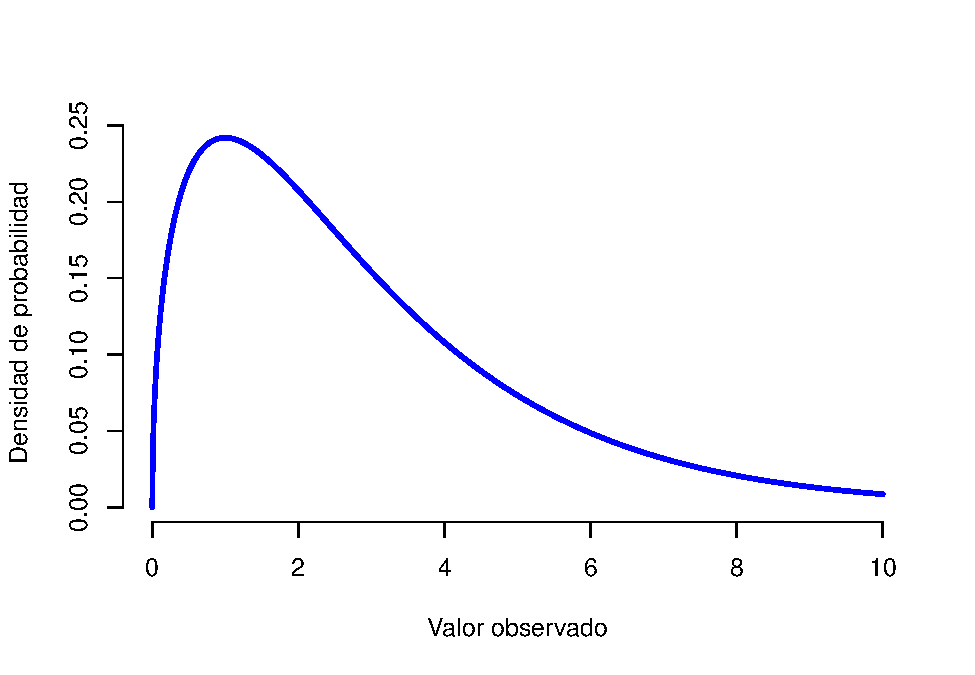
\includegraphics{FdI2_files/figure-latex/chisqdist-1.pdf}
\caption{\label{fig:chisqdist}Una distribución \(chi^2\) con 3 grados de
libertad (3 repeticiones, lo explicaremos más adelante). Observa que los
valores siempre deben ser mayores que cero (los valores se elevan al
cuadrado y se suman), y que la distribución es bastante sesgada (en este
caso hacia la derecha). Estas son las características clave de una
distribución chi-cuadrado.}
\end{figure}

\begin{itemize}
\tightlist
\item
  La \textbf{\emph{distribución \(F\)}} se parece un poco a la
  distribución \(\chi^2\) y surge cada vez que necesitamos comparar dos
  distribuciones \(\chi^2\) entre sí. Es decir, si queremos comparar dos
  ``sumas de cuadrados'' diferentes, nos encontraremos con una
  distribución \(F\). Aún no hemos visto un ejemplo de todo lo que
  implica una suma de cuadrados, pero lo veremos cuando hablemos sobre
  ANOVAs, donde nos encontraremos nuevamente con la distribución \(F\).
\end{itemize}

\begin{figure}
\centering
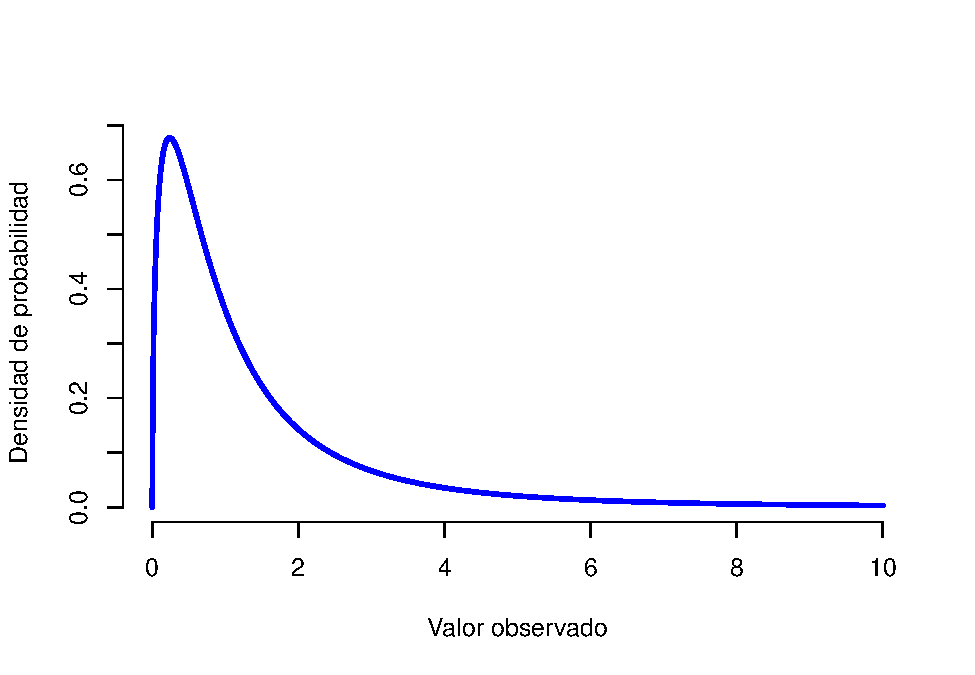
\includegraphics{FdI2_files/figure-latex/Fdist-1.pdf}
\caption{\label{fig:Fdist}Una distribución \(F\) con 3 y 5 grados de
libertad. Cualitativamente hablando, es similar a una distribución de
chi-cuadrado, pero por lo general el significado no es el mismo.}
\end{figure}

Debido a que estas distribuciones están estrechamente relacionadas con
la distribución normal y entre sí, y porque se convertirán en las
distribuciones importantes al hacer análisis estadísticos inferenciales
en este curso, creo que es útil hacer una pequeña demostración de cómo
estas distribuciones realmente están relacionadas entre sí. Primero,
imagina que tenemos un conjunto de 1,000 observaciones aleatorias
distribuidas normalmente al cual llamaremos ``Muestra A''.

Esta ``Muestra A'' es una variable que contiene 1,000 números que se
distribuyen normalmente y tienen una media de 0 y desviación estándar de
1. En la Figura \ref{fig:distnormal} podemos ver un histograma con la
distribución de los valores organizados por columnas, así como una línea
negra sólida que representa la distribución verdadera de los datos (es
decir, una distribución normal con valores infinitos con media 0 y
desviación estándar 1). Así podemos comparar los datos recién generados
con los de una distribución normal verdadera.

\begin{figure}
\centering
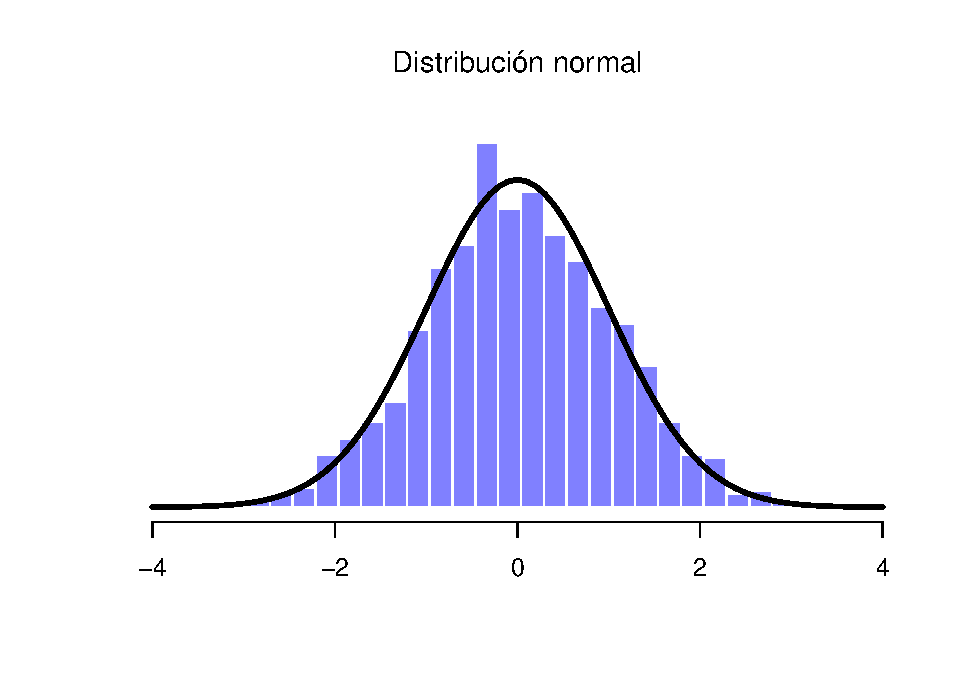
\includegraphics{FdI2_files/figure-latex/distnormal-1.pdf}
\caption{\label{fig:distnormal}Distribución normal de la Muestra A
(histograma), junto con la distribución normal verdadera (línea sólida)}
\end{figure}

En la Figura anterior podemos observar cómo han sido generados muchos
valores distribuidos normalmente que luego han sido comparados con la
distribución de probabilidad verdadera (línea sólida). Supongamos que
ahora queremos una distribución chi-cuadrada con 3 grados de libertad.
Como hemos mencionado anteriormente, una distribución chi-cuadrada con
\(k\) grados de libertad es es el resultado de tomar \(k\) variables (o
muestras) normalmente distribuidas (con media 0 y desviación estándar
1), elevarlas al cuadrado y sumarlas. Como queremos una distribución de
chi-cuadrada con 3 grados de libertad, además de nuestra ``Muestra A'',
necesitamos dos conjuntos más de valores (también distribuidos
normalmente). A estas nuevas dos variables las llamaremos ``Muestra B''
y ``Muestra C'':

\begin{figure}
\centering
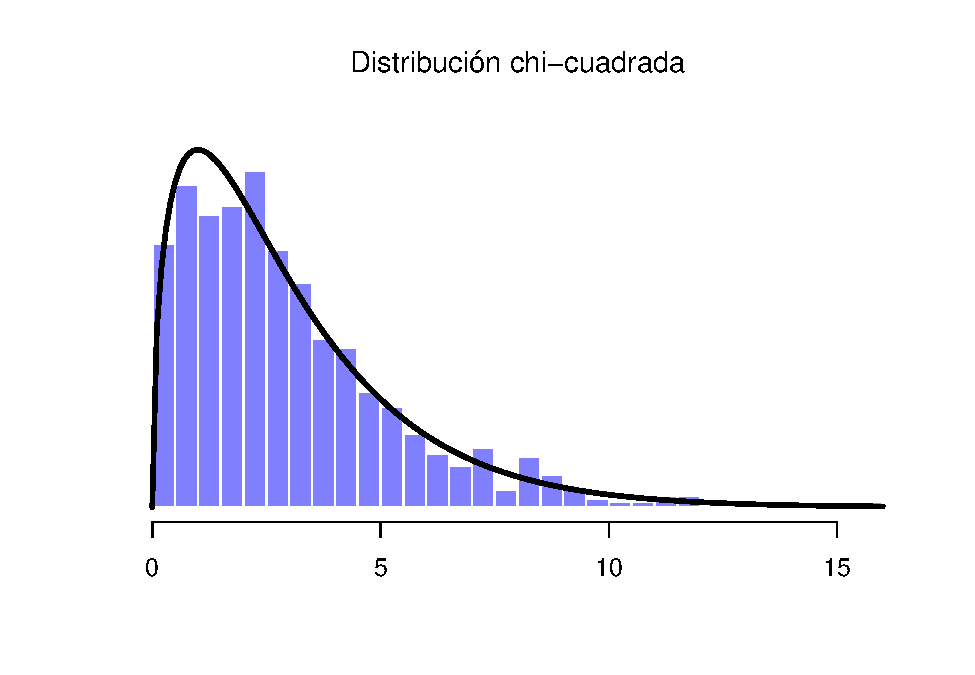
\includegraphics{FdI2_files/figure-latex/distchi-1.pdf}
\caption{\label{fig:distchi}Distribución chi-cuadrada. Incluye a las
Muestras A, B y C (3 grados de libertad)}
\end{figure}

Una vez que tenemos las tres variables, la teoría dice que debemos
elevarlos al cuadrado y sumarlos, con lo que obtendremos 1,000
observaciones que siguen una distribución de chi-cuadrada con 3 grados
de libertad. Visualmente, obtendremos una distribución como en la Figura
\ref{fig:distchi}.

Podemos extender esta demostración y tratar de entender el origen de la
distribución \(t\) y la distribución \(F\). Antes, hemos dicho que la
distribución \(t\) está relacionada con la distribución normal cuando se
desconoce la media o la desviación estándar. Sin embargo, existe una
relación más precisa entre las distribuciones normal, chi-cuadrada y
\(t\). Supongamos que ``escalamos'' nuestros datos anteriores de la
chi-cuadrada al dividirla entre sus 3 grados de libertad.

Si tomamos un conjunto de variables normalmente distribuidas (pensemos
ahora en una ``Muestra D'') y las dividimos por (la raíz cuadrada de)
nuestra variable chi-cuadrada ``escalada'' que tenía \(k=3\) grados de
libertad, la operación dará como resultado una distribución \(t\) con 3
grados de libertad. Si trazamos el histograma de esta nueva distribución
\(t\), observaremos algo parecido al de la Figura \ref{fig:distt}.

\begin{figure}
\centering
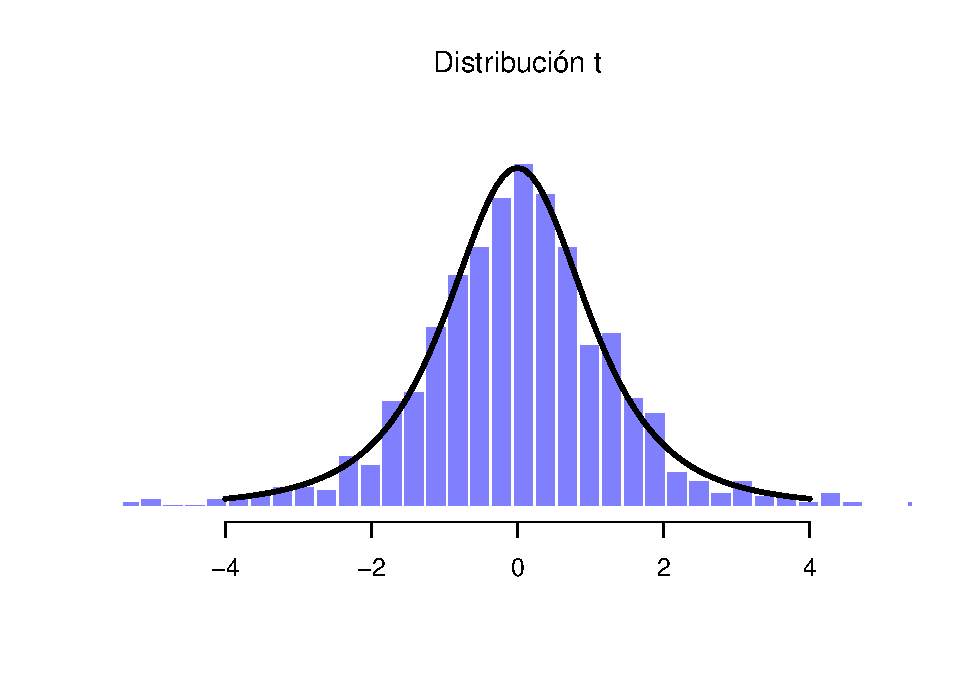
\includegraphics{FdI2_files/figure-latex/distt-1.pdf}
\caption{\label{fig:distt}Distribución t. Es el resultado de dividir una
distribución normal (en este caso la Muestra D) entre una variable
chi-cuadrada escalada}
\end{figure}

Del mismo modo, podemos obtener una distribución \(F\) al dividir dos
distribuciones chi-cuadrada ``escaladas''. Supongamos, por ejemplo, que
deseamos generar datos que sigan una distribución \(F\) con 3 y 20
grados de libertad (es decir, con 3 y 20 variables respectivamente). La
división de los valores de ambas distribuciones nos da como resultado
una nueva variable \texttt{F.3.20} y su distribución es la que se
muestra en la Figura \ref{fig:distf}.

\begin{figure}
\centering
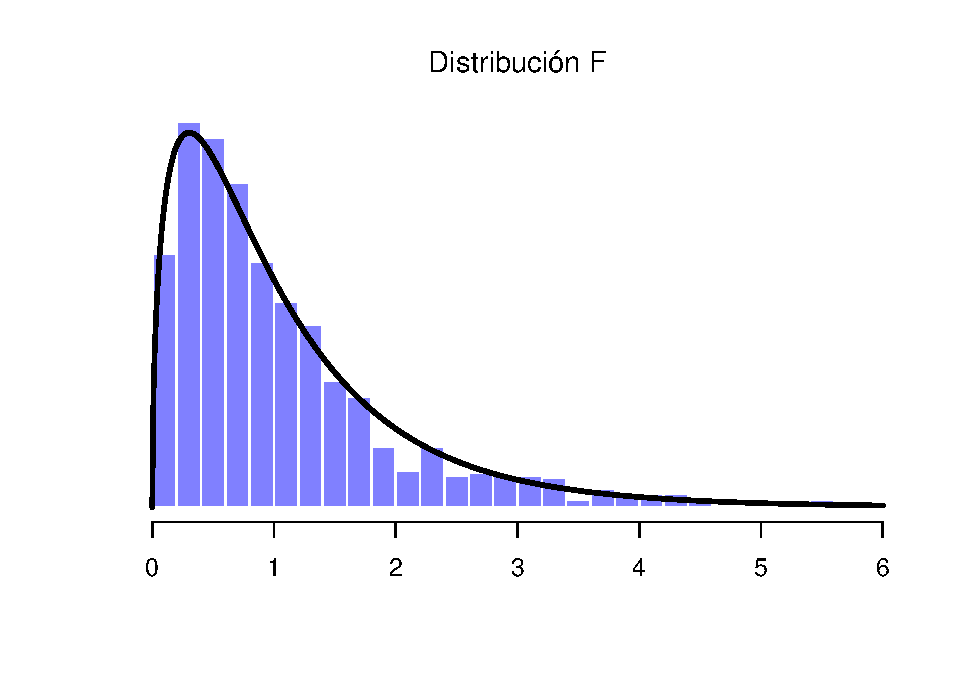
\includegraphics{FdI2_files/figure-latex/distf-1.pdf}
\caption{\label{fig:distf}Distribución F. En este ejemplo hipotético, se
compara la distribución chi-cuadrada de 3 grados de libertad previa con
otra distribución chi-cuadrada con 20 grados de libertad (es decir, que
incluye 20 muestras o variables)}
\end{figure}

Hemos visto tres nuevas distribuciones: \(\chi^2\), \(t\) y \(F\). Todas
son distribuciones continuas, y todas están estrechamente relacionadas
con la distribución normal. Hemos hablado un poco poco sobre la
naturaleza de esta relación. Sin embargo, la clave no es que tengas una
comprensión profunda y detallada de todas estas diferentes
distribuciones, ni que recuerdes las relaciones precisas que existen
entre ellas. Lo más importante es entender la idea básica de que estas
distribuciones están profundamente relacionadas entre sí y a su vez con
la distribución normal. Más adelante en el curso nos vamos a encontrar
con datos que se distribuyen normalmente, o que al menos suponemos que
se distribuyen normalmente. Por lo tanto, si suponemos que nuestros
datos se distribuyen normalmente, debemos saber reconocer las
distribuciones \(\chi^2\), \(t\) y \(F\)..

\section{Resumen}\label{resumen}

En este capítulo hemos hablado de probabilidad. Hemos hablado de lo que
significa la probabilidad y por qué los estadísticos no están muy de
acuerdo en lo que significa. Hablamos sobre las reglas que las
probabilidades tienen que obedecer. Hemos introducido la idea de una
distribución de probabilidad y conocido algunas de las distribuciones de
probabilidad más importantes con las que nos podemos encontrar. Los
temas han sido los siguientes:

\begin{itemize}
\tightlist
\item
  Teoría de probabilidad vs estadística (Sección \ref{probstats})
\item
  Visión frecuenciantista vs visión bayesiana de probabilidad (Sección
  \ref{probmeaning})
\item
  Conceptos básicos de la teoría de probabilidad (Sección
  \ref{basicprobability})
\item
  Distribución binomial (Sección \ref{binomial}), distribución normal
  (sección \ref{normal}), y otras distribuciones (Sección
  \ref{otherdists})
\end{itemize}

Esto es una simple introducción dentro de un gran tema. La teoría de la
probabilidad es una rama de las matemáticas, completamente separada de
su aplicación a la estadística y al análisis de datos. Como tales, hay
miles de libros escritos sobre el tema y las universidades generalmente
ofrecen clases dedicadas por completo a la teoría de la probabilidad. En
este capítulo se han descrito cinco distribuciones de probabilidad
estándar, pero existen \emph{muchas} más que esas. Afortunadamente,
estas distribuciones bastarán por el momento.

Los conceptos básicos que hemos adquirido en este capítulo servirán como
fundamento para los siguientes dos. Existen muchas reglas sobre lo que
se nos ``permite'' decir cuando hacemos inferencia estadística, y muchas
de ellas pueden parecer arbitrarias. Sin embargo, veremos que comienzan
a tener sentido si tenemos en cuenta estos conceptos básicos que hemos
aprendido.

\chapter{Estimando cantidades desconocidas de una
muestra}\label{estimation}

Al comienzo del capítulo inicial, vimos la distinción que existe entre
la \emph{estadística descriptiva} y la \emph{estadística inferencial}.
El papel de la estadística descriptiva es resumir de manera concisa lo
que \emph{ya sabemos}. Por otro lado, el propósito de la estadística
inferencial es ``aprender lo que no sabemos a partir de lo que
hacemos''. Ahora que tenemos cierto conocimiento sobre la teoría de la
probabilidad, podemos pensar en el problema de la inferencia
estadística. ¿Qué tipo de información nos gustaría conocer o aprender?
¿Y cómo lo aprendemo? Estas son las preguntas que se encuentran en el
corazón de la estadística inferencial y tradicionalmente se dividen en
dos ``grandes ideas'': la estimación y la prueba o contraste de
hipótesis. El objetivo de este capítulo es presentar la primera de estas
grandes ideas, la teoría de la estimación. Pero antes, hablaré sobre la
teoría del muestreo, ya que la teoría de la estimación no tiene sentido
hasta que no se comprende el muestreo. Como consecuencia, este capítulo
se divide en dos partes, las secciones \ref{srs} a \ref{samplesandclt}
se centran en la teoría del muestreo, y las secciones
\ref{pointestimates} y \ref{ci} hacen uso de esa teoría del muestreo
para discutir cómo piensan los estadísticos sobre la estimación.

\section{Muestras, poblaciones y muestreo}\label{srs}

Antes hemos hablado sobre el proceso de inducción inferencial, donde
recalcamos que \emph{todo} aprendizaje (o aquello que queremos llegar a
conocer) requiere que hagamos suposiciones. Aceptando que esto es
cierto, hemos de aceptar algunas suposiciones generales sobre los datos
que hemos adquirido para poder utilizarlos. Aquí es donde entra en juego
la \textbf{\emph{teoría del muestreo}}. Si la teoría de la probabilidad
representa los cimientos sobre los que se construye toda la teoría
estadística, la teoría del muestreo es el marco alrededor del cual se
puede construir el resto de la casa. La teoría del muestreo juega un
papel muy importante en la especificación de los supuestos en los que se
basan sus inferencias estadísticas. Y para hablar sobre ``hacer
inferencias'' de la forma en que los estadísticos lo piensan, debemos
ser un poco más explícitos acerca de \emph{qué} es lo que estamos
extrayendo (la muestra) y \emph{sobre qué} es de lo que estamos haciendo
inferencias (la población).

En casi todas las situaciones de interés, lo que tenemos a nuestra
disposición como investigadores es una \emph{muestra} de datos.
Podríamos, por ejemplo, haber realizado un experimento con un cierto
número de participantes; una empresa de encuestas podría haber
telefoneado a algunas personas para hacer preguntas sobre las
intenciones de voto, etc. Independientemente de cual sea el caso, el
conjunto de datos disponibles que tengamos es finito e incompleto. No
podemos conseguir que todas las personas del mundo realicen nuestro
experimento; una empresa de encuestas no tiene el tiempo ni el dinero
para llamar a todos los votantes del país, etc. Para la estadística
descriptiva esta muestra es lo único que importa. Con la estadística
inferencial daremos un paso más allá.

\subsection{Definición de una población}\label{pop}

Una muestra es una cosa muy concreta. Puedes abrir un archivo de Excel y
ahí podrás encontrar los datos de una muestra. Una
\textbf{\emph{población}}, por otro lado, es una idea más abstracta. Se
refiere al conjunto de todas las personas posibles, o todas las
observaciones posibles, sobre las que desea sacar conclusiones y, en
general, es \emph{mucho} más grande que la muestra. En un mundo ideal,
el investigador comenzaría el estudio con una idea clara de cuál es la
población de interés, ya que el proceso de diseñar un estudio y probar
una hipótesis sobre los datos que produce depende de la población sobre
la que se quiere hacer declaraciones. Sin embargo, en la práctica esto
no sucede siempre: por lo general, el investigador tiene una idea
bastante vaga de lo que es la población y diseña el estudio lo mejor que
puede sobre esa base.

A veces es fácil indicar cuál es la población de interés. En el ejemplo
de la ``empresa de encuestas'' que vimos en el capítulo anterior, la
población consistía en todos los votantes inscritos en un momento del
estudio: varios millones de personas. En cambio, la muestra fue un
conjunto de 1000 personas que pertenecen todas a esa población. Sin
embargo, en la mayoría de los casos, esta definición muestra/población
no es tan fácil. En estudios o experimentos con seres humanos,
determinar la población de interés es un poco más complicado. Supongamos
que realizo un experimento con 100 estudiantes de pregrado que
representan mi muestra. Mi objetivo es, por ejemplo, intentar aprender
algo sobre cómo una intervención modifica la dinámica de una clase.
Tomando en cuento a la muestra que tenemos, ¿cuál de las siguientes
opciones contará como ``la población''?:

\begin{itemize}
\tightlist
\item
  ¿Todos los estudiantes de educación de la Universidad de Navarra?\\
\item
  ¿Estudiantes de grado en educación en general, de cualquier parte del
  mundo?\\
\item
  ¿Españoles vivos actualmente?\\
\item
  ¿Españoles de edades similares a las de mi muestra?
\item
  ¿Hispanoparlantes?
\item
  ¿Cualquier persona viva actualmente?\\
\item
  ¿Cualquier ser humano, pasado, presente o futuro?
\end{itemize}

Cada una de estas opciones define un grupo real de personas, las cuales
podrían ser todas de interés para mí como investigador en educación, y
no es tan obvio cuál debería ser la verdadera población de interés.

\subsection{Muestras aleatorias
simples}\label{muestras-aleatorias-simples}

\begin{figure}
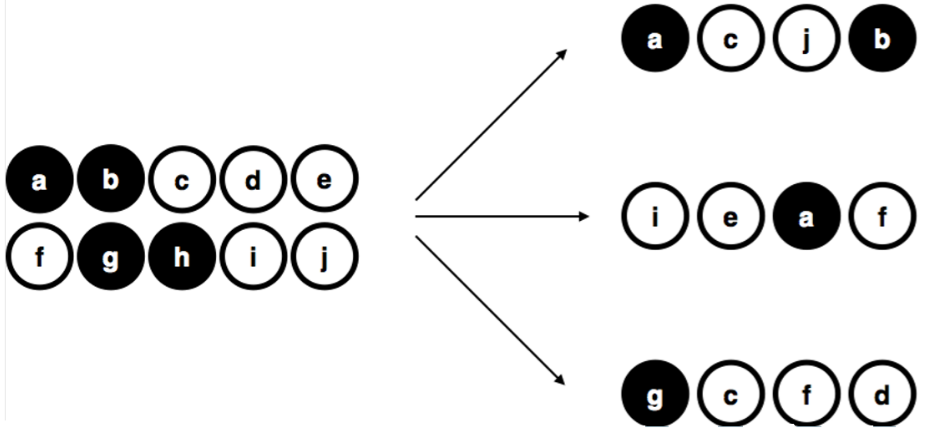
\includegraphics[width=12.86in]{img/estimation/srs1} \caption{Simple random sampling without replacement from a finite population}\label{fig:srs1}
\end{figure}

Independientemente de cómo definamos a una población, la clave es que la
muestra es un subgrupo de esa población, y nuestro objetivo es utilizar
nuestro conocimiento de la muestra para hacer inferencias sobre las
propiedades de la población. La relación que exista entre los dos
dependerá del \emph{procedimiento} mediante el cual se seleccionó la
muestra. Este procedimiento se conoce como \textbf{\emph{método de
muestreo}} y es importante comprender su importancia.

Pongamos un ejemplo sencillo. Imaginemos que tenemos una bolsa que
contiene 10 fichas. Cada ficha tiene una letra única impresa, por lo que
la podemos distinguir de entre las otras 10 fichas. Las fichas vienen en
dos colores, blanco y negro. Este conjunto de fichas es la población de
interés y se muestra gráficamente a la izquierda de la Figura
\ref{fig:srs1}. Como podrás ver en la imagen, tenemos 4 fichas negras y
6 fichas blancas, pero recuerda que en la vida real esto no lo sabríamos
a menos que miráramos en la bolsa. Ahora imagina que realizas el
siguiente ``experimento'': agitas la bolsa, cierras los ojos y sacas 4
fichas sin devolver ninguna de ellas a la bolsa. Primero sale la ficha
\(a\) (negra), seguida de la ficha \(c\) (blanca), luego la \(j\)
(blanca) y finalmente la ficha \(b\) (negra). Una vez extraídas 4
fichas, podrás volver a poner todas las fichas en la bolsa y repetir el
experimento, como se muestra en el lado derecho de la Figura
\ref{fig:srs1}. Cada vez que repites el experimento obtienes resultados
diferentes, pero el procedimiento es idéntico en cada caso. El hecho de
que el mismo procedimiento pueda dar lugar a resultados diferentes cada
vez, lo define como un proceso \emph{aleatorio}. Y debido a que hemos
agitado la bolsa antes de sacar las fichas, parece razonable pensar que
todas las fichas tienen las mismas posibilidades de ser seleccionadas.
Un procedimiento en el que todos los miembros de la población tienen las
mismas posibilidades de ser seleccionados se denomina
\textbf{\emph{muestra aleatoria simple}}. El hecho de que se \emph{no}
se devuelvan las fichas a la bolsa después de salir, significa que no
podremos observar la misma ficha dos veces, y en tales casos se dice que
ha habido un muestreo \textbf{\emph{sin reemplazo}}.

Para comprender la importancia del procedimiento de muestreo,
consideremos ahora una forma alternativa en la que podría haberse
realizado el experimento. Supongamos que mi sobrino de 3 años coge la
bolsa y decide sacar las cuatro fichas negras (le gusta el color negro)
sin devolverlas la bolsa. Este esquema de muestreo \emph{sesgado} se
muestra en la Figura \ref{fig:brs}. Ahora considera el valor que tiene
obtener una muestra con 4 fichas negras y 0 fichas blancas siguiendo el
procedimiento de mi sobrino. Vemos pues, como el valor dependerá mucho
del método de muestreo. Si sabemos que el método de muestreo está
sesgado para seleccionar únicamente fichas negras, entonces una muestra
que consta únicamente de fichas negras no dice mucho sobre nuestra
población de fichas. Por esta razón, los estadísticos prefieren que un
conjunto de datos provenga de una muestra aleatoria simple, ya que
facilita \emph{mucho} el análisis de los datos.

\begin{figure}
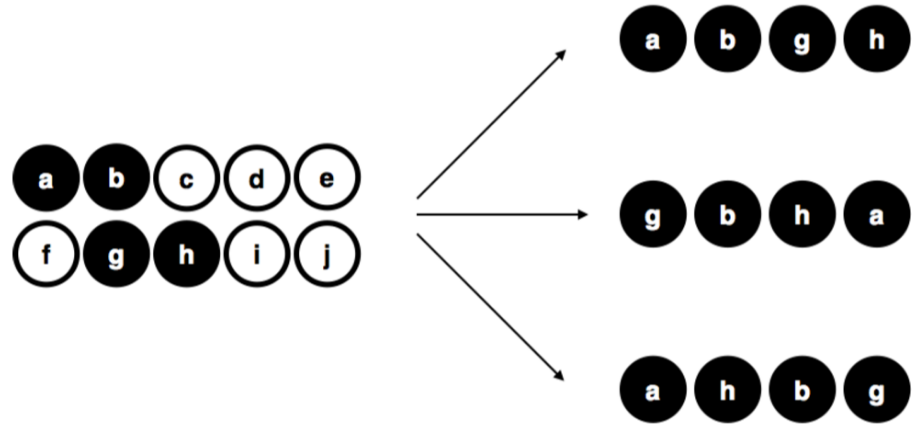
\includegraphics[width=12.81in]{img/estimation/brs} \caption{Biased sampling without replacement from a finite population}\label{fig:brs}
\end{figure}

\begin{figure}
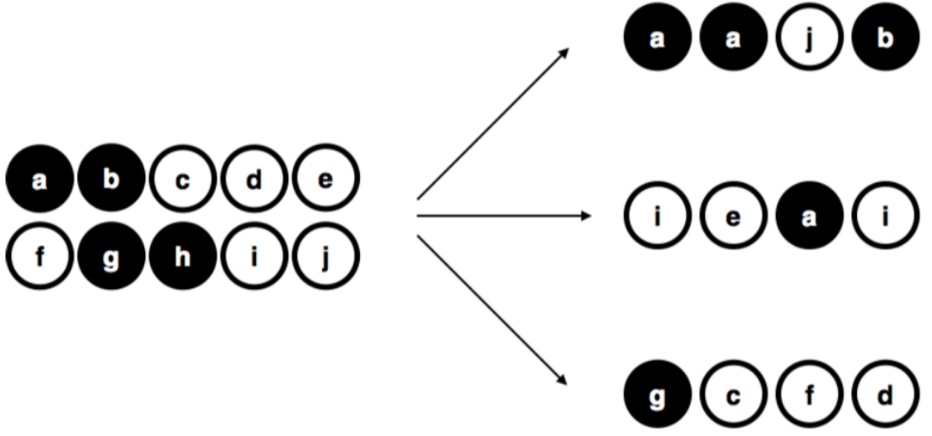
\includegraphics[width=12.94in]{img/estimation/srs2} \caption{Simple random sampling *with* replacement from a finite population}\label{fig:srs2}
\end{figure}

Vale la pena mencionar un tercer procedimiento. Esta vez cerramos los
ojos, agitamos la bolsa y sacamos una ficha. Sin embargo, esta vez
registramos la observación y luego volvemos a poner la ficha dentro de
la bolsa. Nuevamente, cerramos los ojos, agitamos la bolsa y sacamos
otra ficha. Repetimos este procedimiento hasta que tengamos 4 fichas.
Los conjuntos de datos que hemos generado de esta manera siguen siendo
muestras aleatorias simples, pero debido a que volvemos a meter las
fichas dentro de la bolsa inmediatamente después de haberlas sacado, se
denomina como una muestra \textbf{\emph{con reemplazo}}. La diferencia
entre este caso y el primero es que es posible observar al mismo
elemento de la población varias veces (en este caso la misma ficha), tal
como se ilustra en la Figura \ref{fig:srs2}.

Por lo general, la mayoría de los experimentos que veamos en ciencias de
la educación tienden a tomar muestras sin reemplazo, ya que la misma
persona no puede participar en el experimento dos veces. Sin embargo,
una gran parte de la teoría estadística se basa en el supuesto de que
los datos surgen de una muestra aleatoria simple \emph{con} reemplazo.
En la vida real, esto rara vez importa. Si la población de interés es
grande, la diferencia entre el muestreo con y sin reemplazo es demasiado
pequeña como para preocuparnos. Sin embargo, la diferencia que existe
entre muestras aleatorias simples y muestras sesgadas no es algo no es
aglo que podemos ignorar tan facilmente.

\subsection{La mayoría de las muestras no son muestras aleatorias
simples}\label{la-mayoria-de-las-muestras-no-son-muestras-aleatorias-simples}

Si miras la lista anterior de posibles poblaciones, te darás cuenta que
es casi imposible obtener una muestra aleatoria simple de la mayoría de
esas poblaciones de interés. Cuando hacemos experimentos con estudiantes
universitarios, el obtener una verdadera muestra aleatoria de estos
estudiantes los podemos considerar como un milagro menor, aunque al
final se trate de una población muy específica a partir de la cual
generalizar. Mencionaré brevemente algunos de los otros tipos de
muestreo que existen y que solemos encontrar con bastante frecuencia:

\begin{itemize}
\item
  \emph{Muestreo estratificado}. Supongamos que tu población está (o
  puede estar) dividida en varias subpoblaciones o \emph{estratos}
  diferentes. Quizás sea porque estás realizando un estudio en varios
  paises diferentes, por ejemplo. En lugar de intentar tomar una muestra
  aleatoria de toda la población en su conjunto, recolectamos una
  muestra aleatoria de cada uno de las subpoblaciones o estratos. El
  muestreo estratificado suele ser más fácil de llevar a cabo que el
  muestreo aleatorio simple, especialmente cuando la población ya está
  dividida en los distintos estratos. También puede ser más eficiente
  que el muestreo aleatorio simple, especialmente cuando algunas de las
  subpoblaciones son raras o poco frecuentes. Por ejemplo, en el estudio
  de la esquizofrenia, resulta más sencillo dividir la población en dos
  estratos (con-esquizofrenia y sin-esquizofrenia) y adquirir una
  muestra de cada grupo. Si seleccionaramos personas al azar,
  obtendríamos tan pocas personas con esquizofrenia en la muestra que el
  estudio resultaría inútil.
\item
  \emph{Muestreo de bola de nieve}. Es una técnica que es especialmente
  útil cuando se toman muestras de una población ``oculta'' o de difícil
  acceso, y es especialmente común en las ciencias sociales. Por
  ejemplo, supongamos que los investigadores quieren realizar una
  encuesta de opinión a personas VIH positivo. Es posible que el equipo
  de investigación solo tenga los datos de contacto de algunas personas
  VIH positivo, por lo que la encuesta comienza pidiéndoles a esas
  personas que participen (etapa 1). Al final de la encuesta, se pide a
  los participantes que proporcionen los datos de contacto de otras
  personas que podrían querer participar. En la etapa 2, se encuesta a
  estos nuevos contactos. El proceso continúa hasta que los
  investigadores obtengan datos suficientes. La gran ventaja del
  muestreo de bola de nieve es que es capaz de proporcionar datos en
  situaciones que de otro modo serían imposibles de obtener. Desde el
  punto de vista estadístico, la principal desventaja es que la muestra
  es altamente no aleatoria y no aleatoria en formas que son difíciles
  de abordar.
\item
  \emph{Muestreo de conveniencia}. En este tipo de muestreo las muestras
  se eligen de una forma conveniente para el investigador, sin que
  exista una selección al azar a partir de la población de interés. El
  muestreo de bola de nieve es un tipo de muestreo de conveniencia, pero
  hay muchos otros. Un ejemplo son los estudios que se basan en
  estudiantes de universitarios. Estas muestras generalmente no son
  aleatorias desde dos puntos de vista: en primer lugar, depender de una
  muestra de estudiantes universitarios significa automáticamente que
  estos datos están restringidos a una sola subpoblación. En segundo
  lugar, los estudiantes suelen elegir los estudios en los que
  participan, por lo que la muestra es un subconjunto de estudiantes
  autoseleccionado, no un subconjunto seleccionado al azar. En general,
  la mayoría de los estudios incluyen muestras de conveniencia de una
  forma u otra. A veces, puede suponer una limitación en la
  interpretación de los resultados, pero no siempre.
\end{itemize}

\subsection{¿Cuánto importa si no tiene una muestra aleatoria
simple?}\label{cuanto-importa-si-no-tiene-una-muestra-aleatoria-simple}

Hemos visto que en muchos casos no es posible recolectar muestras
aleatorias simples. ¿Eso qué impacto tiene? Un ejemplo de ese impacto lo
podemos apreciar con la diferencia que existe entre las Figuras
\ref{fig:srs1} y \ref{fig:brs}. Sin embargo, no es tan malo como parece.
Algunos tipos de muestras sesgadas no representan ningún problema. Por
ejemplo, cuando utilizamos el muestreo estratificado, realmente sabemos
\emph{cuál} es el sesgo ya que lo hemos creado deliberadamente, con la
intención de \emph{aumentar} la efectividad de su estudio, y existen
técnicas estadísticas que podemos utilizar para ajustar estos sesgos que
hemos introducido. En estos casos, por lo tanto, no tenemos un problema.

Sin embargo, es importante recordar que el muestreo aleatorio es un
medio para un fin, no el fin en sí mismo. Supongamos que recolectamos
una muestra de conveniencia y, como tal, podemos asumir que está
sesgada. Un sesgo en el método de muestreo solo es un problema si nos
hace sacar conclusiones equivocadas. Desde esta perspectiva, podemos
afirmar que no necesitamos que la muestra sea aleatoria en \emph{todos}
los aspectos: necesitamos que sea aleatoria con respecto al fenómeno de
interés que buscamos estudiar. Supongamos que estoy haciendo un estudio
sobre la capacidad de atención sostenida en niños de 6 años. En el
estudio 1, tengo la capacidad de tomar muestras al azar de todos los
niños de 6 años del mundo actualmente vivos, con una pequeña excepción:
sólo puedo incluir niños nacidos en lunes. En el estudio 2, puedo tomar
una muestra al azar de la población española. Con estos estudios quiero
generalizar mis resultados a la población de todos los niños de 6 años.
¿Qué estudio es mejor? La respuesta, obviamente, es el estudio 1. ¿Por
qué? Porque no tenemos ninguna razón para pensar que ``nacer en lunes''
influye en la capacidad de atención sostenida. Por otro lado, puedo
pensar en varias razones por las que ``ser español'' podría ser
importante. España es un país rico e industrializado con un sistema
educativo muy desarrollado. Las personas que crecieron con este sistema
habrán tenido experiencias de vida mucho más similares a las
experiencias de vida de las personas que diseñaron las pruebas de
capacidad de atención sostenida. Esta experiencia compartida podría
traducirse fácilmente en creencias similares sobre cómo se debe
``realizar una prueba'', entre otros. Este tipo de características son
importantes y pueden, por ejemplo, llevar a una imagen engañosa de lo
que es la capacidad atención sostenida.

Existe un reflexión clave oculta en esta discusión. Al diseñar estudios,
es importante pensar en la población de interés y en esforzarse por
elegir un método de muestreo que sea apropiado para esa población. En la
práctica, muchas veces nos veremos obligados a utilizar una ``muestra de
conveniencia'' (por ejemplo, estudiantes de unos pocos centros), pero
deberíamos, al menos, dedicar un tiempo a pensar en los riesgos e
implicaciones de esta práctica.

\subsection{Parámetros poblacionales y estadísticos
muestrales}\label{parametros-poblacionales-y-estadisticos-muestrales}

Hasta ahora hemos estado hablando de poblaciones como lo haría un
científico. Para un educador, una población puede ser un grupo de niños.
Para un ecologista, una población puede ser un grupo de osos. En la
mayoría de los casos, las poblaciones son cosas concretas que realmente
existen en el mundo real. Los estadísticos, sin embargo, tienen un
interés dual. Por un lado, \emph{están} interesados en los datos del
mundo real de la misma forma que los científicos. Por otro lado, también
operan en el ámbito de la abstracción pura como lo hacen los
matemáticos. En consecuencia, la teoría estadística puede ser un poco
abstracta cuando define una población. Para ello, los estadísticos
operacionalizan el concepto de ``población'' en términos de objetos
matemáticos los cuales ya conocemos: se llaman distribuciones de
probabilidad.

La idea es muy simple. Digamos que estamos hablando (otra vez) de
puntajes de coeficiente intelectual (CI). Para un educador, la población
de interés es un grupo de humanos reales que tienen puntajes de CI. Un
estadístico ``simplifica'' esto al definir operativamente a la población
como la distribución de probabilidad representada en la Figura
\ref{fig:IQdista}. Las pruebas de CI están \emph{diseñadas} de tal forma
que la media sea 100, que la desviación estándar sea 15 y que la
distribución de los puntajes sea normal. Estos valores se denominan
\textbf{\emph{parámetros poblacionales}} porque son característicos de
toda la población. Es decir, decimos que la media de la población
\(\mu\) es 100, y la desviación estándar de la población \(\sigma\) es
15.

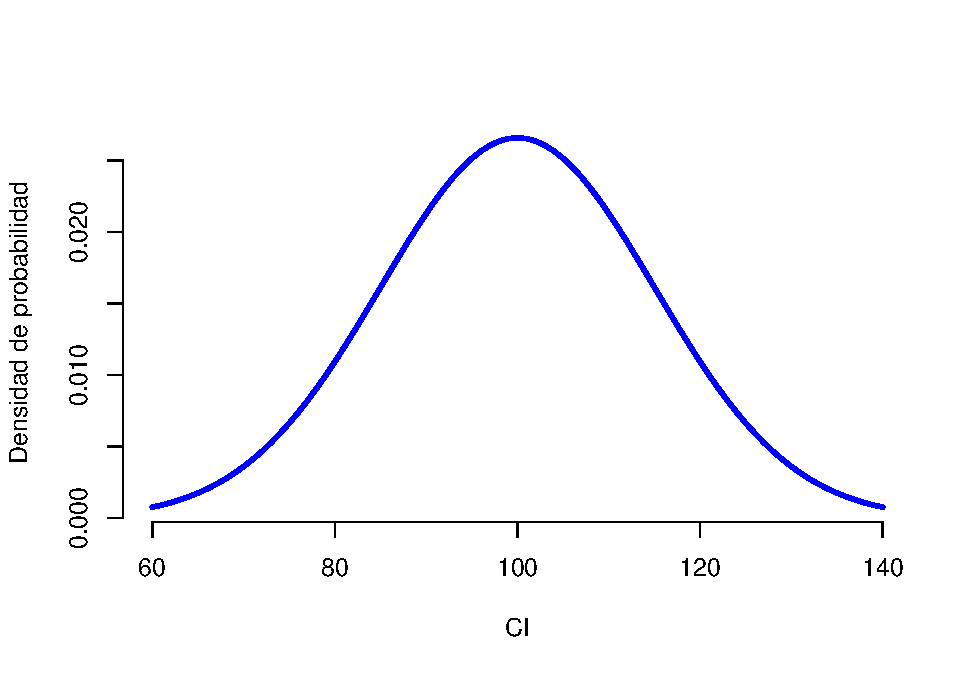
\includegraphics{FdI2_files/figure-latex/IQdist-1.pdf}
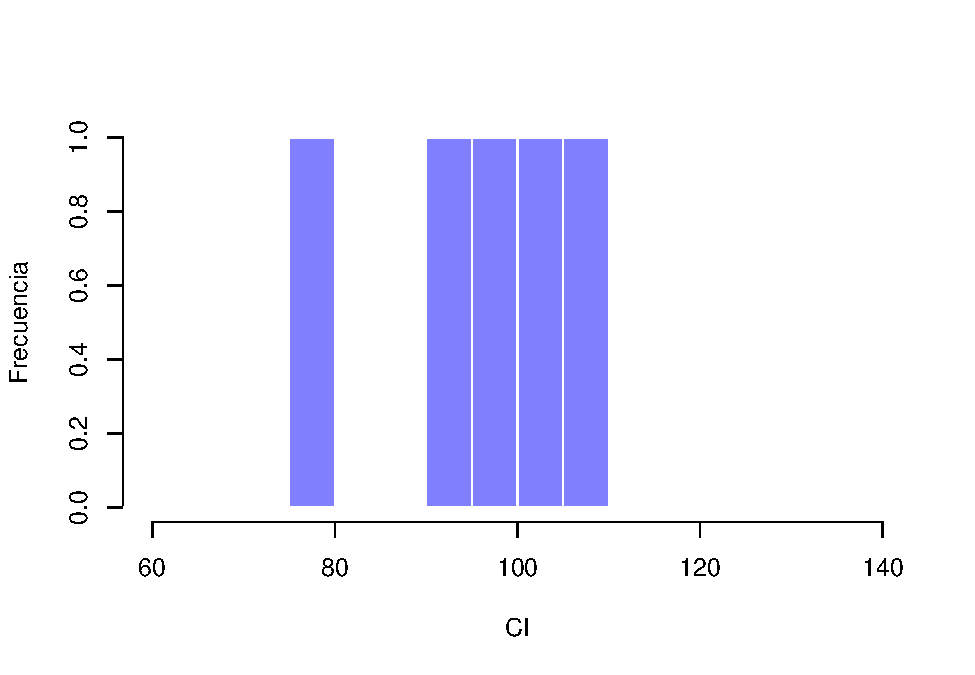
\includegraphics{FdI2_files/figure-latex/IQdist-2.pdf}

\begin{verbatim}
## [1] "n= 5 mean= 95.0439814361422 sd= 15.8950870458079"
\end{verbatim}

\begin{figure}
\centering
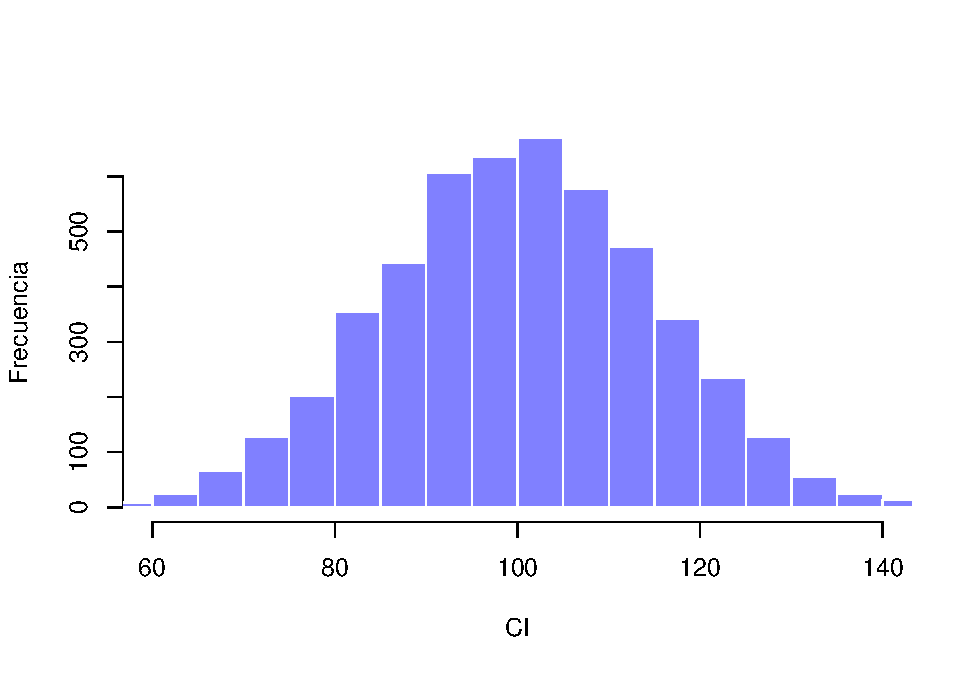
\includegraphics{FdI2_files/figure-latex/IQdist-3.pdf}
\caption{\label{fig:IQdist3}Distribución poblacional de los puntajes de CI
(Panel A) y dos muestra extraídas de forma aleatoria de esta población.
En el Panel B una muestra con 100 observaciones y en el Panel C una
muestra con 10,000 observaciones.}
\end{figure}

\begin{verbatim}
## [1] "n= 5000 mean= 100.001142624934 sd= 15.115479046001"
\end{verbatim}

Supongamos que hacemos un experimento. Seleccionamos 100 personas al
azar para que elaboren nuestro test de CI, lo cual me dará una muestra
aleatoria de la población. Mi muestra consistirá de una serie de números
como estos:

\begin{verbatim}
                          106 101 98 80 74 ... 107 72 100
\end{verbatim}

Estos puntajes son una muestra extraída de una población con
distribución norma, media de 100 y desviación estándar de 15. Si
trazamos un histograma de esta muestra, obtendremos algo como el que se
muestra en la Figura \ref{fig:IQdist}b. Podemos ver que el histograma
tiene una forma \emph{aproximadamente} normal, pero aún queda como una
aproximación burda de la verdadera distribución de la población que se
muestra en la Figura \ref{fig:IQdist}a. Si calculamos la media muestral,
obtendremos un número que está bastante cerca de la media de la
población 100, pero no es idéntico. En este caso, vemos que las personas
de mi muestra tienen un CI medio de 98,5 y la desviación estándar de sus
puntuaciones de CI es de 15,9. Estos \textbf{\emph{estadísticos
muestrales}} nos presentan una descripción de nuestro conjunto de datos
y, aunque son bastante similares a los valores reales de población, no
son iguales. En general, los estadísticos muestrales son lo que podemos
calcular a partir de un conjunto de datos mientras que los parámetros
poblacionales son las cosas sobre las que deseamos aprender. Más
adelante, hablaremos sobre cómo podemos estimar los parámetros
poblacionales utilizando sus estadísticos muestrales (Sección
\ref{pointestimates}) así como qué tan seguros estamos de esos
estimadores (Sección \ref{ci}) pero antes necesitamos conocer algunos
conceptos adicionales sobre la teoría de muestreo.

\section{La ley de los grandes números}\label{lawlargenumbers}

En la sección anterior vimos los resultados de un experimento ficticio
con un tamaño de muestra de \(N=100\). Los resultados fueron algo
alentadores: la media real de la población es 100 y la media muestral
98.5, una aproximación razonable. En muchos estudios científicos, este
nivel de precisión es perfectamente aceptable, pero existen situaciones
en las que nos gustaría ser bastante más precisos. Si queremos que
nuestros estadísticos muestrales se acerquen más a los parámetros
poblaciones, ¿qué podemos hacer al respecto?

La respuesta lógica sería recolectar más datos. Supongamos que hacemos
un experimento más grande, en el cual medimos el CI de 10,000 personas.
Si entrás \href{https://leudave.shinyapps.io/sampling/}{aquí} podrás
hacer una simulación. El histograma de esta simulación se muestra en la
Figura \ref{fig:IQdist}c. Una inspección rápida nos revelará que una
muestra de mayor tamaño es representa una mucho mejor aproximación la
distribución poblacional real, especialmente si la comparamos con la
muestra más pequeña. Esto también se ve reflejado en los estadísticos
muestrales: el CI medio de la muestra grande es de 99.9 y su desviación
estándar es de 15.1. Estos valores son muy cercanos a los valores reales
de la población.

Con esto, podemos observar algo que parece obvio: entre más datos
tengamos, mejores resultados obtendremos. Esta intuición tan evidente
que compartimos todos, los estadísticos la definen como la
\textbf{\emph{ley de los grandes números}}. La ley de los grandes
números es una ley matemática que aplica a muchos estadísticos
muestrales, pero la forma más sencilla de entenderla es a través de la
ley aplicada a las medias. Cuando se aplica a la media muestral, la ley
de los grande números nos dice que conforme aumenta el tamaño de
muestra, el valor de la media muestral se acercará al valor de la media
poblacional real. O, para ser más precisos, conforme el tamaño muestral
se aproxima al infinito (escrito como \(N \rightarrow \infty\)) la media
nuestral se aproximará a la media poblacional
(\(\bar{X} \rightarrow \mu\)).\footnote{Técnicamente, la de ley de los
  grandes números es aplicable a cualquier estadístico muestral que
  pueda ser descrito como un promedio de cantidades independiente. La
  varianza muestral, por ejemplo, puede ser representado como un tipo de
  promedio y por ello, sujeto a la ley de los grandes números. Sin
  embargo, el valor mínimo muestral no puede ser interpretado como un
  promedio de nada, y por tanto, no es gobernado por la ley de los
  grandes números.}

Espero que quede patente la importancia de la ley de los grandes números
como una herramienta elemental en la teoría estadística. Esta ley de los
grandes números es nuestro argumento para justificar nuestra creencia de
que recolectar cada vez más y más datos nos acercará a la verdad. Para
cualquier conjunto de datos, los estadísticos muestrales que calculemos
estarán equivocados, pero la ley de los grandes números nos dice que si
seguimos recolectando datos esos estadísticos muestrales tenderán a a
acerca más y más a los parámetros poblacionales reales.

\section{Distribuciones muestrales y el teorema del límite
central}\label{samplesandclt}

La ley de los grandes números es una herramienta muy poderosa, pero no
será suficiente para responder a todas nuestras preguntas. Entre otras
cosas, lo que nos da esta ley es una ``garantía a largo plazo''. A largo
plazo, si pudiéramos recolectar una cantidad infinita de datos, la ley
de los grandes números nos garantiza que los estadísticos muestrales
serán correctos.

Sin embargo, esta ``garantía a largo plazo'' es de poca utilidad en la
vida real: no basta con decir que \emph{con el tiempo} llegaremos a la
respuesta correcta cuando calculemos la media muestral. Saber que un
conjunto de datos infinitamente largo me dará el valor exacto de la
media poblacional es inconciliable con el \emph{hecho} de que mi
conjunto de datos tiene un tamaño de muestra de \(N=100\). En la vida
real, tenemos que saber algo más sobre el comportamiento de la media
muestral de una muestra modesta como la nuestra.

\subsection{Distribución muestral de la media}\label{samplingdists}

Abandonemos por un momento la idea de tener tamaños de muestra de 10,000
y pensemos en un experimento más modesto (y realista). Esta vez
extraemos una muestra de \(N=5\) personas y medimos su CI. Este es el
resultado:

\begin{verbatim}
90  82  94  99 110
\end{verbatim}

El CI medio de esta muestra es exactamente 95. Esta muestra nos revela
un valor mucho menos preciso que en el experimento previo. Ahora imagina
que decides \textbf{\emph{replicar}} este mismo experimento. Es decir,
quieres repetir el mismo procedimiento de tal forma que selecciones una
nueva muestra aleatoria de 5 personas y obtener su CI una vez más. Estos
son los CI de nuestra nueva muestra:

\begin{verbatim}
78  88 111 111 117
\end{verbatim}

Al calcular la media de esta muestra vemos que es de 101. Si repetimos
el experimento 10 veces más obtendremos los resultados que se muestran
en la Tabla \ref{tab:replications}. Con ella podrás que la media muestra
cambia con cada replicación del experimento.

\begin{tabular}{l|r|r|r|r|r|r}
\hline
. & P1 & P2 & P3 & P4 & P5 & Media.Muestral\\
\hline
Rep 1 & 90 & 82 & 94 & 99 & 110 & 95.0\\
\hline
Rep 2 & 78 & 88 & 111 & 111 & 117 & 101.0\\
\hline
Rep 3 & 111 & 122 & 91 & 98 & 86 & 101.6\\
\hline
Rep 4 & 98 & 96 & 119 & 99 & 107 & 103.8\\
\hline
Rep 5 & 105 & 113 & 103 & 103 & 98 & 104.4\\
\hline
Rep 6 & 81 & 89 & 93 & 85 & 114 & 92.4\\
\hline
Rep 7 & 100 & 93 & 108 & 98 & 133 & 106.4\\
\hline
Rep 8 & 107 & 100 & 105 & 117 & 85 & 102.8\\
\hline
Rep 9 & 86 & 119 & 108 & 73 & 116 & 100.4\\
\hline
Rep 10 & 95 & 126 & 112 & 120 & 76 & 105.8\\
\hline
\end{tabular}

Supongamos ahora que decidimos continuar con este procedimiento,
replicando el experimento de ``5 puntuaciones de CI'' una y otra vez. Y
cada vez, obtendremos una media muestra diferente, que en el caso de los
10 experimentos que ya hemos hecho corresponderían con los siguientes
valores:

\begin{verbatim}
                      95.0 101.0 101.6 103.8 104.4 ...
\end{verbatim}

¿Qué pasaría si continuamos y recolectamos 10,000 medias muestrales y
trazamos un histograma con ellas? Obtendríamos un resultado como el que
vemos en la Figura \ref{fig:sampdistmean}. En esta imagen podemos
apreciar que la media muestral de 5 puntuaciones de CI se encuentra, por
lo general, entre 90 y 110. Pero lo más interesante de esta Figura es
que demuestra el hecho de que si repetimos el experimento una y otra
vez, ¡lo que obtenemos es una \emph{distribución} de las medias
muestrales! Esta distribución recibe un nombre especial en estadística:
se le llama \textbf{\emph{distribución muestral de la media}}.

La distribuciones muestrales

Las distribuciones muestrales son una idea teórica importante en la
estadística, y además, son cruciales si queremos entender cómo se
comportan las muestras pequeñas. Por ejempo, cuando realizamos el primer
experimento con 5 puntuaciones de CI, la media muestral fue de 95. Sin
embargo, lo que la distribución muestral nos dice en la Figura
\ref{fig:sampdistmean}, es que este experimento con 5 puntuaciones no es
muy preciso. Si repetimos el experimento muchas veces, la distribución
muestral nos dice que podemos esperar que la media muestral esté entre
80 y 120.

\begin{figure}
\centering
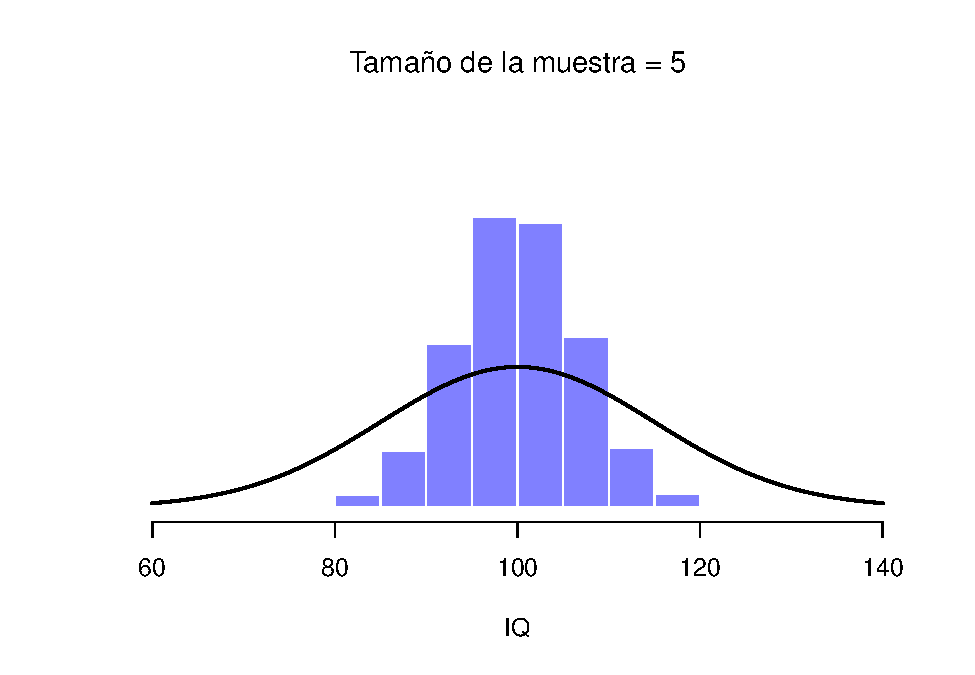
\includegraphics{FdI2_files/figure-latex/sampdistmean-1.pdf}
\caption{\label{fig:sampdistmean}La distribución muestral de la media en el
experimento con 5 puntuaciones de CI. Si obtenemos una muestra aleatoria
de 5 personas y calculamos la \emph{media} de sus puntajes, obtendremos
casi con seguridad un valor entre 80 y 120, aunque existen individuos
que tienen un CI mayor de 120 o menor de 80. La línea negra dibuja la
distribución poblacional de los puntajes de CI para comparar.}
\end{figure}

\subsection{Sampling distributions exist for any sample
statistic!}\label{sampling-distributions-exist-for-any-sample-statistic}

One thing to keep in mind when thinking about sampling distributions is
that \emph{any} sample statistic you might care to calculate has a
sampling distribution. For example, suppose that each time I replicated
the ``five IQ scores'' experiment I wrote down the largest IQ score in
the experiment. This would give me a data set that started out like
this:

\begin{verbatim}
                      110 117 122 119 113 ... 
\end{verbatim}

Doing this over and over again would give me a very different sampling
distribution, namely the \emph{sampling distribution of the maximum}.
The sampling distribution of the maximum of 5 IQ scores is shown in
Figure \ref{fig:sampdistmax}. Not surprisingly, if you pick 5 people at
random and then find the person with the highest IQ score, they're going
to have an above average IQ. Most of the time you'll end up with someone
whose IQ is measured in the 100 to 140 range.

\subsection{The central limit theorem}\label{clt}

An illustration of the how sampling distribution of the mean depends on
sample size. In each panel, I generated 10,000 samples of IQ data, and
calculated the mean IQ observed within each of these data sets. The
histograms in these plots show the distribution of these means (i.e.,
the sampling distribution of the mean). Each individual IQ score was
drawn from a normal distribution with mean 100 and standard deviation
15, which is shown as the solid black line).

\begin{figure}
\centering
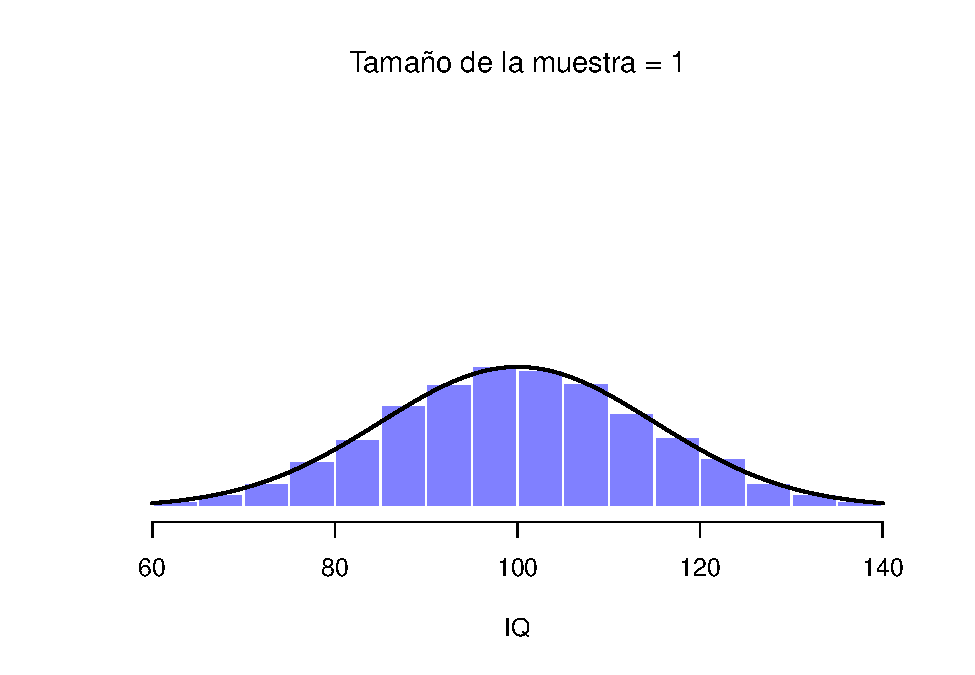
\includegraphics{FdI2_files/figure-latex/IQsampa-1.pdf}
\caption{\label{fig:IQsampa}Each data set contained only a single
observation, so the mean of each sample is just one person's IQ score.
As a consequence, the sampling distribution of the mean is of course
identical to the population distribution of IQ scores.}
\end{figure}

\begin{figure}
\centering
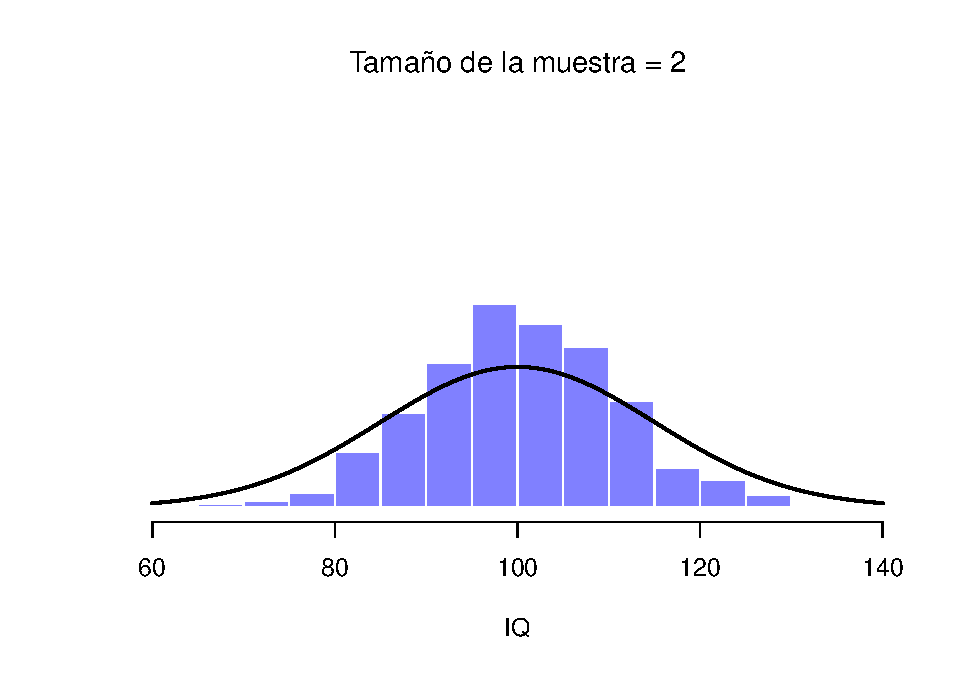
\includegraphics{FdI2_files/figure-latex/IQsampb-1.pdf}
\caption{\label{fig:IQsampb}When we raise the sample size to 2, the mean of
any one sample tends to be closer to the population mean than a one
person's IQ score, and so the histogram (i.e., the sampling
distribution) is a bit narrower than the population distribution.}
\end{figure}

\begin{figure}
\centering
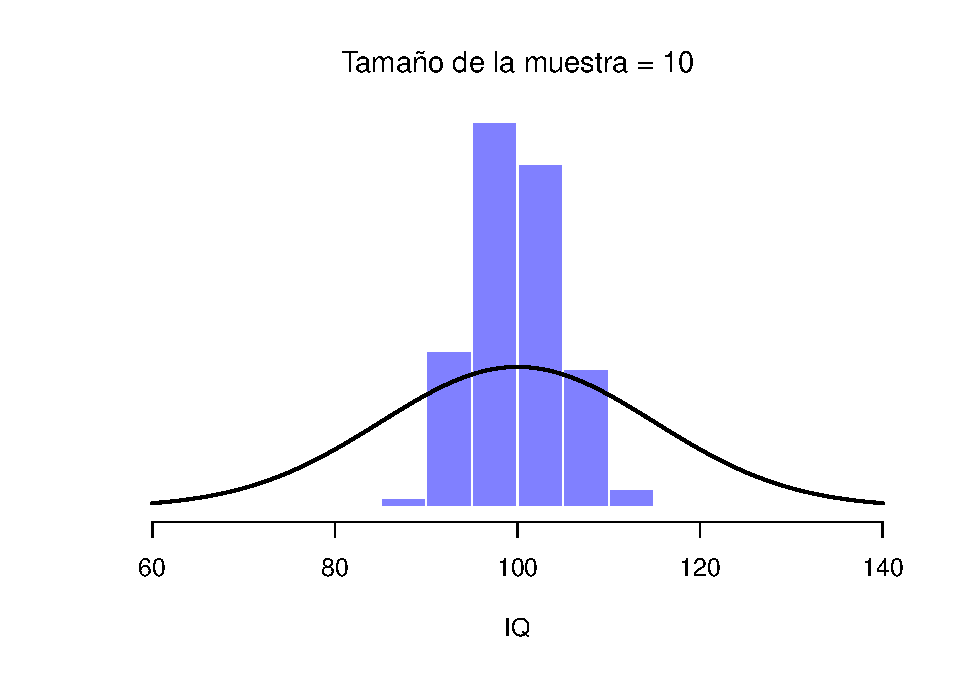
\includegraphics{FdI2_files/figure-latex/IQsampc-1.pdf}
\caption{\label{fig:IQsampc}By the time we raise the sample size to 10, we
can see that the distribution of sample means tend to be fairly tightly
clustered around the true population mean.}
\end{figure}

At this point I hope you have a pretty good sense of what sampling
distributions are, and in particular what the sampling distribution of
the mean is. In this section I want to talk about how the sampling
distribution of the mean changes as a function of sample size.
Intuitively, you already know part of the answer: if you only have a few
observations, the sample mean is likely to be quite inaccurate: if you
replicate a small experiment and recalculate the mean you'll get a very
different answer. In other words, the sampling distribution is quite
wide. If you replicate a large experiment and recalculate the sample
mean you'll probably get the same answer you got last time, so the
sampling distribution will be very narrow. You can see this visually in
Figures \ref{fig:IQsampa}, \ref{fig:IQsampb} and \ref{fig:IQsampc}: the
bigger the sample size, the narrower the sampling distribution gets. We
can quantify this effect by calculating the standard deviation of the
sampling distribution, which is referred to as the
\textbf{\emph{standard error}}. The standard error of a statistic is
often denoted SE, and since we're usually interested in the standard
error of the sample \emph{mean}, we often use the acronym SEM. As you
can see just by looking at the picture, as the sample size \(N\)
increases, the SEM decreases.

Okay, so that's one part of the story. However, there's something I've
been glossing over so far. All my examples up to this point have been
based on the ``IQ scores'' experiments, and because IQ scores are
roughly normally distributed, I've assumed that the population
distribution is normal. What if it isn't normal? What happens to the
sampling distribution of the mean? The remarkable thing is this: no
matter what shape your population distribution is, as \(N\) increases
the sampling distribution of the mean starts to look more like a normal
distribution. To give you a sense of this, I ran some simulations using
R. To do this, I started with the ``ramped'' distribution shown in the
histogram in Figure \ref{fig:cltdemo}. As you can see by comparing the
triangular shaped histogram to the bell curve plotted by the black line,
the population distribution doesn't look very much like a normal
distribution at all. Next, I used R to simulate the results of a large
number of experiments. In each experiment I took \(N=2\) samples from
this distribution, and then calculated the sample mean. Figure
\ref{fig:cltdemob} plots the histogram of these sample means (i.e., the
sampling distribution of the mean for \(N=2\)). This time, the histogram
produces a \(\cap\)-shaped distribution: it's still not normal, but it's
a lot closer to the black line than the population distribution in
Figure \ref{fig:cltdemoa}. When I increase the sample size to \(N=4\),
the sampling distribution of the mean is very close to normal (Figure
\ref{fig:cltdemoc}, and by the time we reach a sample size of \(N=8\)
it's almost perfectly normal. In other words, as long as your sample
size isn't tiny, the sampling distribution of the mean will be
approximately normal no matter what your population distribution looks
like!

\begin{Shaded}
\begin{Highlighting}[]
    \CommentTok{# needed for printing}
\NormalTok{    width <-}\StringTok{ }\DecValTok{6}
\NormalTok{    height <-}\StringTok{ }\DecValTok{6} 
    
    \CommentTok{# parameters of the beta}
\NormalTok{    a <-}\StringTok{ }\DecValTok{2}
\NormalTok{    b <-}\StringTok{ }\DecValTok{1}
    
    \CommentTok{# mean and standard deviation of the beta}
\NormalTok{    s <-}\StringTok{ }\KeywordTok{sqrt}\NormalTok{( a}\OperatorTok{*}\NormalTok{b }\OperatorTok{/}\StringTok{ }\NormalTok{(a}\OperatorTok{+}\NormalTok{b)}\OperatorTok{^}\DecValTok{2} \OperatorTok{/}\StringTok{ }\NormalTok{(a}\OperatorTok{+}\NormalTok{b}\OperatorTok{+}\DecValTok{1}\NormalTok{) )}
\NormalTok{    m <-}\StringTok{ }\NormalTok{a }\OperatorTok{/}\StringTok{ }\NormalTok{(a}\OperatorTok{+}\NormalTok{b)}
    
    \CommentTok{# define function to draw a plot}
\NormalTok{    plotOne <-}\StringTok{ }\ControlFlowTok{function}\NormalTok{(n,}\DataTypeTok{N=}\DecValTok{10000}\NormalTok{) \{}
        
        \CommentTok{# generate N random sample means of size n}
\NormalTok{        X <-}\StringTok{ }\KeywordTok{matrix}\NormalTok{(}\KeywordTok{rbeta}\NormalTok{(n}\OperatorTok{*}\NormalTok{N,a,b),n,N)}
\NormalTok{        X <-}\StringTok{ }\KeywordTok{colMeans}\NormalTok{(X)}
        
        \CommentTok{# plot the data}
        \KeywordTok{hist}\NormalTok{( X, }\DataTypeTok{breaks=}\KeywordTok{seq}\NormalTok{(}\DecValTok{0}\NormalTok{,}\DecValTok{1}\NormalTok{,.}\DecValTok{025}\NormalTok{), }\DataTypeTok{border=}\StringTok{"white"}\NormalTok{, }\DataTypeTok{freq=}\OtherTok{FALSE}\NormalTok{,}
            \DataTypeTok{col=}\KeywordTok{ifelse}\NormalTok{(colour,emphColLight,emphGrey),}
            \DataTypeTok{xlab=}\StringTok{"Media muestral"}\NormalTok{, }\DataTypeTok{ylab=}\StringTok{""}\NormalTok{, }\DataTypeTok{xlim=}\KeywordTok{c}\NormalTok{(}\DecValTok{0}\NormalTok{,}\FloatTok{1.2}\NormalTok{),}
            \DataTypeTok{main=}\KeywordTok{paste}\NormalTok{(}\StringTok{"Tamaño de la muestra ="}\NormalTok{,n), }\DataTypeTok{axes=}\OtherTok{FALSE}\NormalTok{,}
            \DataTypeTok{font.main=}\DecValTok{1}\NormalTok{, }\DataTypeTok{ylim=}\KeywordTok{c}\NormalTok{(}\DecValTok{0}\NormalTok{,}\DecValTok{12}\NormalTok{)}
\NormalTok{        )}
        \KeywordTok{box}\NormalTok{()}
        \KeywordTok{axis}\NormalTok{(}\DecValTok{1}\NormalTok{)}
        \CommentTok{#axis(2)}
        
        \CommentTok{# plot the theoretical distribution}
        \KeywordTok{lines}\NormalTok{( x <-}\StringTok{ }\KeywordTok{seq}\NormalTok{(}\DecValTok{0}\NormalTok{,}\FloatTok{1.2}\NormalTok{,.}\DecValTok{01}\NormalTok{), }\KeywordTok{dnorm}\NormalTok{(x,m,s}\OperatorTok{/}\KeywordTok{sqrt}\NormalTok{(n)), }
            \DataTypeTok{lwd=}\DecValTok{2}\NormalTok{, }\DataTypeTok{col=}\StringTok{"black"}\NormalTok{, }\DataTypeTok{type=}\StringTok{"l"}
\NormalTok{        )}
\NormalTok{    \}}
    
    \ControlFlowTok{for}\NormalTok{( i }\ControlFlowTok{in} \KeywordTok{c}\NormalTok{(}\DecValTok{50}\NormalTok{)) \{}
        \KeywordTok{plotOne}\NormalTok{(i)\}}
\end{Highlighting}
\end{Shaded}

\begin{figure}
\centering
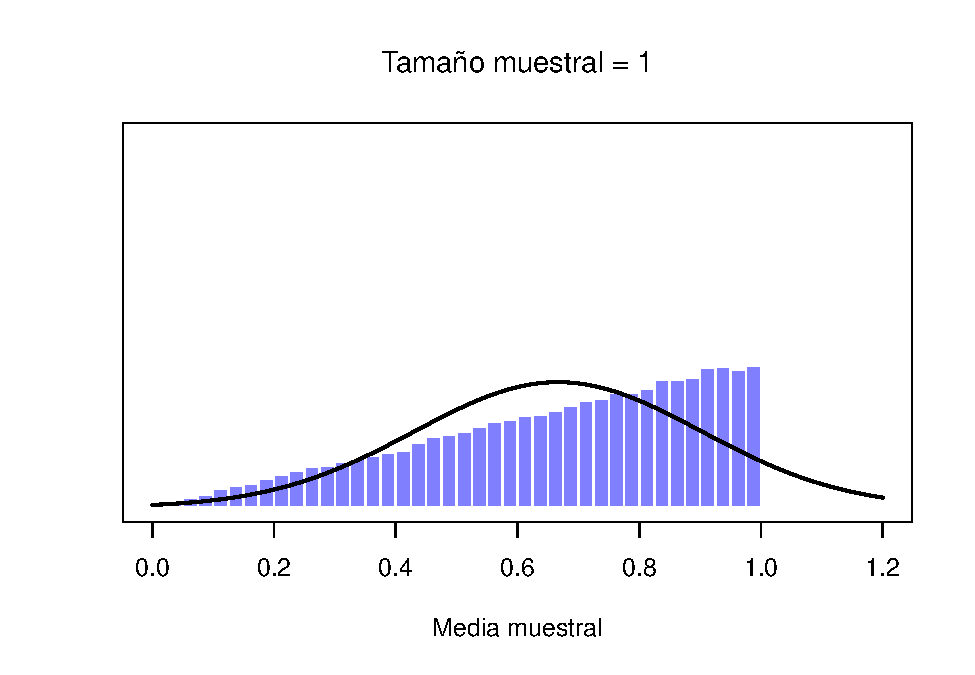
\includegraphics{FdI2_files/figure-latex/cltdemo-1.pdf}
\caption{\label{fig:cltdemo}A demonstration of the central limit theorem. In
panel a, we have a non-normal population distribution; and panels b-d
show the sampling distribution of the mean for samples of size 2,4 and
8, for data drawn from the distribution in panel a. As you can see, even
though the original population distribution is non-normal, the sampling
distribution of the mean becomes pretty close to normal by the time you
have a sample of even 4 observations.}
\end{figure}

On the basis of these figures, it seems like we have evidence for all of
the following claims about the sampling distribution of the mean:

\begin{itemize}
\tightlist
\item
  The mean of the sampling distribution is the same as the mean of the
  population
\item
  The standard deviation of the sampling distribution (i.e., the
  standard error) gets smaller as the sample size increases
\item
  The shape of the sampling distribution becomes normal as the sample
  size increases
\end{itemize}

As it happens, not only are all of these statements true, there is a
very famous theorem in statistics that proves all three of them, known
as the \textbf{\emph{central limit theorem}}. Among other things, the
central limit theorem tells us that if the population distribution has
mean \(\mu\) and standard deviation \(\sigma\), then the sampling
distribution of the mean also has mean \(\mu\), and the standard error
of the mean is \[
\mbox{SEM} = \frac{\sigma}{ \sqrt{N} }
\] Because we divide the population standard devation \(\sigma\) by the
square root of the sample size \(N\), the SEM gets smaller as the sample
size increases. It also tells us that the shape of the sampling
distribution becomes normal.\footnote{As usual, I'm being a bit sloppy
  here. The central limit theorem is a bit more general than this
  section implies. Like most introductory stats texts, I've discussed
  one situation where the central limit theorem holds: when you're
  taking an average across lots of independent events drawn from the
  same distribution. However, the central limit theorem is much broader
  than this. There's a whole class of things called ``\(U\)-statistics''
  for instance, all of which satisfy the central limit theorem and
  therefore become normally distributed for large sample sizes. The mean
  is one such statistic, but it's not the only one.}

This result is useful for all sorts of things. It tells us why large
experiments are more reliable than small ones, and because it gives us
an explicit formula for the standard error it tells us \emph{how much}
more reliable a large experiment is. It tells us why the normal
distribution is, well, \emph{normal}. In real experiments, many of the
things that we want to measure are actually averages of lots of
different quantities (e.g., arguably, ``general'' intelligence as
measured by IQ is an average of a large number of ``specific'' skills
and abilities), and when that happens, the averaged quantity should
follow a normal distribution. Because of this mathematical law, the
normal distribution pops up over and over again in real data.

\section{Estimating population parameters}\label{pointestimates}

In all the IQ examples in the previous sections, we actually knew the
population parameters ahead of time. As every undergraduate gets taught
in their very first lecture on the measurement of intelligence, IQ
scores are \emph{defined} to have mean 100 and standard deviation 15.
However, this is a bit of a lie. How do we know that IQ scores have a
true population mean of 100? Well, we know this because the people who
designed the tests have administered them to very large samples, and
have then ``rigged'' the scoring rules so that their sample has mean
100. That's not a bad thing of course: it's an important part of
designing a psychological measurement. However, it's important to keep
in mind that this theoretical mean of 100 only attaches to the
population that the test designers used to design the tests. Good test
designers will actually go to some lengths to provide ``test norms''
that can apply to lots of different populations (e.g., different age
groups, nationalities etc).

This is very handy, but of course almost every research project of
interest involves looking at a different population of people to those
used in the test norms. For instance, suppose you wanted to measure the
effect of low level lead poisoning on cognitive functioning in Port
Pirie, a South Australian industrial town with a lead smelter. Perhaps
you decide that you want to compare IQ scores among people in Port Pirie
to a comparable sample in Whyalla, a South Australian industrial town
with a steel refinery.\footnote{Please note that if you were
  \emph{actually} interested in this question, you would need to be a
  \emph{lot} more careful than I'm being here. You \emph{can't} just
  compare IQ scores in Whyalla to Port Pirie and assume that any
  differences are due to lead poisoning. Even if it were true that the
  only differences between the two towns corresponded to the different
  refineries (and it isn't, not by a long shot), you need to account for
  the fact that people already \emph{believe} that lead pollution causes
  cognitive deficits: if you recall back to Chapter \ref{studydesign},
  this means that there are different demand effects for the Port Pirie
  sample than for the Whyalla sample. In other words, you might end up
  with an illusory group difference in your data, caused by the fact
  that people \emph{think} that there is a real difference. I find it
  pretty implausible to think that the locals wouldn't be well aware of
  what you were trying to do if a bunch of researchers turned up in Port
  Pirie with lab coats and IQ tests, and even less plausible to think
  that a lot of people would be pretty resentful of you for doing it.
  Those people won't be as co-operative in the tests. Other people in
  Port Pirie might be \emph{more} motivated to do well because they
  don't want their home town to look bad. The motivational effects that
  would apply in Whyalla are likely to be weaker, because people don't
  have any concept of ``iron ore poisoning'' in the same way that they
  have a concept for ``lead poisoning''. Psychology is \emph{hard}.}
Regardless of which town you're thinking about, it doesn't make a lot of
sense simply to \emph{assume} that the true population mean IQ is 100.
No-one has, to my knowledge, produced sensible norming data that can
automatically be applied to South Australian industrial towns. We're
going to have to \textbf{\emph{estimate}} the population parameters from
a sample of data. So how do we do this?

\subsection{Estimating the population
mean}\label{estimating-the-population-mean}

Suppose we go to Port Pirie and 100 of the locals are kind enough to sit
through an IQ test. The average IQ score among these people turns out to
be \(\bar{X}=98.5\). So what is the true mean IQ for the entire
population of Port Pirie? Obviously, we don't know the answer to that
question. It could be \(97.2\), but if could also be \(103.5\). Our
sampling isn't exhaustive so we cannot give a definitive answer.
Nevertheless if I was forced at gunpoint to give a ``best guess'' I'd
have to say \(98.5\). That's the essence of statistical estimation:
giving a best guess.

In this example, estimating the unknown poulation parameter is
straightforward. I calculate the sample mean, and I use that as my
\textbf{\emph{estimate of the population mean}}. It's pretty simple, and
in the next section I'll explain the statistical justification for this
intuitive answer. However, for the moment what I want to do is make sure
you recognise that the sample statistic and the estimate of the
population parameter are conceptually different things. A sample
statistic is a description of your data, whereas the estimate is a guess
about the population. With that in mind, statisticians often different
notation to refer to them. For instance, if true population mean is
denoted \(\mu\), then we would use \(\hat\mu\) to refer to our estimate
of the population mean. In contrast, the sample mean is denoted
\(\bar{X}\) or sometimes \(m\). However, in simple random samples, the
estimate of the population mean is identical to the sample mean: if I
observe a sample mean of \(\bar{X} = 98.5\), then my estimate of the
population mean is also \(\hat\mu = 98.5\). To help keep the notation
clear, here's a handy table:

\begin{Shaded}
\begin{Highlighting}[]
\NormalTok{knitr}\OperatorTok{::}\KeywordTok{kable}\NormalTok{(}\KeywordTok{data.frame}\NormalTok{(}\DataTypeTok{stringsAsFactors=}\OtherTok{FALSE}\NormalTok{,}
                   \DataTypeTok{Symbol =} \KeywordTok{c}\NormalTok{(}\StringTok{"$}\CharTok{\textbackslash{}\textbackslash{}}\StringTok{bar\{X\}$"}\NormalTok{, }\StringTok{"$}\CharTok{\textbackslash{}\textbackslash{}}\StringTok{mu$"}\NormalTok{, }\StringTok{"$}\CharTok{\textbackslash{}\textbackslash{}}\StringTok{hat\{}\CharTok{\textbackslash{}\textbackslash{}}\StringTok{mu\}$"}\NormalTok{),}
              \DataTypeTok{What.is.it =} \KeywordTok{c}\NormalTok{(}\StringTok{"Sample mean"}\NormalTok{, }\StringTok{"True population mean"}\NormalTok{,}
                              \StringTok{"Estimate of the population mean"}\NormalTok{),}
   \DataTypeTok{Do.we.know.what.it.is =} \KeywordTok{c}\NormalTok{(}\StringTok{"Yes  calculated from the raw data"}\NormalTok{,}
                              \StringTok{"Almost never known for sure"}\NormalTok{,}
                              \StringTok{"Yes  identical to the sample mean"}\NormalTok{)))}
\end{Highlighting}
\end{Shaded}

\begin{tabular}{l|l|l}
\hline
Symbol & What.is.it & Do.we.know.what.it.is\\
\hline
\$\textbackslash{}bar\{X\}\$ & Sample mean & Yes  calculated from the raw data\\
\hline
\$\textbackslash{}mu\$ & True population mean & Almost never known for sure\\
\hline
\$\textbackslash{}hat\{\textbackslash{}mu\}\$ & Estimate of the population mean & Yes  identical to the sample mean\\
\hline
\end{tabular}

\subsection{Estimating the population standard
deviation}\label{estimating-the-population-standard-deviation}

So far, estimation seems pretty simple, and you might be wondering why I
forced you to read through all that stuff about sampling theory. In the
case of the mean, our estimate of the population parameter (i.e.
\(\hat\mu\)) turned out to identical to the corresponding sample
statistic (i.e. \(\bar{X}\)). However, that's not always true. To see
this, let's have a think about how to construct an
\textbf{\emph{estimate of the population standard deviation}}, which
we'll denote \(\hat\sigma\). What shall we use as our estimate in this
case? Your first thought might be that we could do the same thing we did
when estimating the mean, and just use the sample statistic as our
estimate. That's almost the right thing to do, but not quite.

Here's why. Suppose I have a sample that contains a single observation.
For this example, it helps to consider a sample where you have no
intutions at all about what the true population values might be, so
let's use something completely fictitious. Suppose the observation in
question measures the \emph{cromulence} of my shoes. It turns out that
my shoes have a cromulence of 20. So here's my sample:

\begin{verbatim}
20
\end{verbatim}

This is a perfectly legitimate sample, even if it does have a sample
size of \(N=1\). It has a sample mean of 20, and because every
observation in this sample is equal to the sample mean (obviously!) it
has a sample standard deviation of 0. As a description of the
\emph{sample} this seems quite right: the sample contains a single
observation and therefore there is no variation observed within the
sample. A sample standard deviation of \(s = 0\) is the right answer
here. But as an estimate of the \emph{population} standard deviation, it
feels completely insane, right? Admittedly, you and I don't know
anything at all about what ``cromulence'' is, but we know something
about data: the only reason that we don't see any variability in the
\emph{sample} is that the sample is too small to display any variation!
So, if you have a sample size of \(N=1\), it \emph{feels} like the right
answer is just to say ``no idea at all''.

Notice that you \emph{don't} have the same intuition when it comes to
the sample mean and the population mean. If forced to make a best guess
about the population mean, it doesn't feel completely insane to guess
that the population mean is 20. Sure, you probably wouldn't feel very
confident in that guess, because you have only the one observation to
work with, but it's still the best guess you can make.

Let's extend this example a little. Suppose I now make a second
observation. My data set now has \(N=2\) observations of the cromulence
of shoes, and the complete sample now looks like this:

\begin{verbatim}
20, 22
\end{verbatim}

This time around, our sample is \emph{just} large enough for us to be
able to observe some variability: two observations is the bare minimum
number needed for any variability to be observed! For our new data set,
the sample mean is \(\bar{X}=21\), and the sample standard deviation is
\(s=1\). What intuitions do we have about the population? Again, as far
as the population mean goes, the best guess we can possibly make is the
sample mean: if forced to guess, we'd probably guess that the population
mean cromulence is 21. What about the standard deviation? This is a
little more complicated. The sample standard deviation is only based on
two observations, and if you're at all like me you probably have the
intuition that, with only two observations, we haven't given the
population ``enough of a chance'' to reveal its true variability to us.
It's not just that we suspect that the estimate is \emph{wrong}: after
all, with only two observations we expect it to be wrong to some degree.
The worry is that the error is \emph{systematic}. Specifically, we
suspect that the sample standard deviation is likely to be smaller than
the population standard deviation.

This intuition feels right, but it would be nice to demonstrate this
somehow. There are in fact mathematical proofs that confirm this
intuition, but unless you have the right mathematical background they
don't help very much. Instead, what I'll do is use R to simulate the
results of some experiments. With that in mind, let's return to our IQ
studies. Suppose the true population mean IQ is 100 and the standard
deviation is 15. I can use the \texttt{rnorm()} function to generate the
the results of an experiment in which I measure \(N=2\) IQ scores, and
calculate the sample standard deviation. If I do this over and over
again, and plot a histogram of these sample standard deviations, what I
have is the \emph{sampling distribution of the standard deviation}. I've
plotted this distribution in Figure \ref{fig:sampdistsd}. Even though
the true population standard deviation is 15, the average of the
\emph{sample} standard deviations is only 8.5. Notice that this is a
very different result to what we found in Figure \ref{fig:IQsampb} when
we plotted the sampling distribution of the mean. If you look at that
sampling distribution, what you see is that the population mean is 100,
and the average of the sample means is also 100.

Now let's extend the simulation. Instead of restricting ourselves to the
situation where we have a sample size of \(N=2\), let's repeat the
exercise for sample sizes from 1 to 10. If we plot the average sample
mean and average sample standard deviation as a function of sample size,
you get the results shown in Figure \ref{fig:estimatorbias}. On the left
hand side (panel a), I've plotted the average sample mean and on the
right hand side (panel b), I've plotted the average standard deviation.
The two plots are quite different: \emph{on average}, the average sample
mean is equal to the population mean. It is an \textbf{\emph{unbiased
estimator}}, which is essentially the reason why your best estimate for
the population mean is the sample mean.\footnote{I should note that I'm
  hiding something here. Unbiasedness is a desirable characteristic for
  an estimator, but there are other things that matter besides bias.
  However, it's beyond the scope of this book to discuss this in any
  detail. I just want to draw your attention to the fact that there's
  some hidden complexity here.} The plot on the right is quite
different: on average, the sample standard deviation \(s\) is
\emph{smaller} than the population standard deviation \(\sigma\). It is
a \textbf{\emph{biased estimator}}. In other words, if we want to make a
``best guess'' \(\hat\sigma\) about the value of the population standard
deviation \(\sigma\), we should make sure our guess is a little bit
larger than the sample standard deviation \(s\).

The fix to this systematic bias turns out to be very simple. Here's how
it works. Before tackling the standard deviation, let's look at the
variance. If you recall from Section \ref{var}, the sample variance is
defined to be the average of the squared deviations from the sample
mean. That is: \[
s^2 = \frac{1}{N} \sum_{i=1}^N (X_i - \bar{X})^2
\] The sample variance \(s^2\) is a biased estimator of the population
variance \(\sigma^2\). But as it turns out, we only need to make a tiny
tweak to transform this into an unbiased estimator. All we have to do is
divide by \(N-1\) rather than by \(N\). If we do that, we obtain the
following formula: \[
\hat\sigma^2 = \frac{1}{N-1} \sum_{i=1}^N (X_i - \bar{X})^2 
\] This is an unbiased estimator of the population variance \(\sigma\).
Moreover, this finally answers the question we raised in Section
\ref{var}. Why did R give us slightly different answers when we used the
\texttt{var()} function? Because the \texttt{var()} function calculates
\(\hat\sigma^2\) not \(s^2\), that's why. A similar story applies for
the standard deviation. If we divide by \(N-1\) rather than \(N\), our
estimate of the population standard deviation becomes: \[
\hat\sigma = \sqrt{\frac{1}{N-1} \sum_{i=1}^N (X_i - \bar{X})^2} 
\] and when we use R's built in standard deviation function
\texttt{sd()}, what it's doing is calculating \(\hat\sigma\), not
\(s\).\footnote{Okay, I'm hiding something else here. In a bizarre and
  counterintuitive twist, since \(\hat\sigma^2\) is an unbiased
  estimator of \(\sigma^2\), you'd assume that taking the square root
  would be fine, and \(\hat\sigma\) would be an unbiased estimator of
  \(\sigma\). Right? Weirdly, it's not. There's actually a subtle, tiny
  bias in \(\hat\sigma\). This is just bizarre: \(\hat\sigma^2\) is and
  unbiased estimate of the population variance \(\sigma^2\), but when
  you take the square root, it turns out that \(\hat\sigma\) is a biased
  estimator of the population standard deviation \(\sigma\). Weird,
  weird, weird, right? So, why is \(\hat\sigma\) biased? The technical
  answer is ``because non-linear transformations (e.g., the square root)
  don't commute with expectation'', but that just sounds like gibberish
  to everyone who hasn't taken a course in mathematical statistics.
  Fortunately, it doesn't matter for practical purposes. The bias is
  small, and in real life everyone uses \(\hat\sigma\) and it works just
  fine. Sometimes mathematics is just annoying.}

One final point: in practice, a lot of people tend to refer to
\(\hat{\sigma}\) (i.e., the formula where we divide by \(N-1\)) as the
\emph{sample} standard deviation. Technically, this is incorrect: the
\emph{sample} standard deviation should be equal to \(s\) (i.e., the
formula where we divide by \(N\)). These aren't the same thing, either
conceptually or numerically. One is a property of the sample, the other
is an estimated characteristic of the population. However, in almost
every real life application, what we actually care about is the estimate
of the population parameter, and so people always report \(\hat\sigma\)
rather than \(s\). This is the right number to report, of course, it's
that people tend to get a little bit imprecise about terminology when
they write it up, because ``sample standard deviation'' is shorter than
``estimated population standard deviation''. It's no big deal, and in
practice I do the same thing everyone else does. Nevertheless, I think
it's important to keep the two \emph{concepts} separate: it's never a
good idea to confuse ``known properties of your sample'' with ``guesses
about the population from which it came''. The moment you start thinking
that \(s\) and \(\hat\sigma\) are the same thing, you start doing
exactly that.

To finish this section off, here's another couple of tables to help keep
things clear:

\begin{Shaded}
\begin{Highlighting}[]
\NormalTok{knitr}\OperatorTok{::}\KeywordTok{kable}\NormalTok{(}\KeywordTok{data.frame}\NormalTok{(}\DataTypeTok{stringsAsFactors=}\OtherTok{FALSE}\NormalTok{,}
                   \DataTypeTok{Symbol =} \KeywordTok{c}\NormalTok{(}\StringTok{"$s$"}\NormalTok{, }\StringTok{"$}\CharTok{\textbackslash{}\textbackslash{}}\StringTok{sigma$"}\NormalTok{, }\StringTok{"$}\CharTok{\textbackslash{}\textbackslash{}}\StringTok{hat\{}\CharTok{\textbackslash{}\textbackslash{}}\StringTok{sigma\}$"}\NormalTok{, }\StringTok{"$s^2$"}\NormalTok{,}
                              \StringTok{"$}\CharTok{\textbackslash{}\textbackslash{}}\StringTok{sigma^2$"}\NormalTok{, }\StringTok{"$}\CharTok{\textbackslash{}\textbackslash{}}\StringTok{hat\{}\CharTok{\textbackslash{}\textbackslash{}}\StringTok{sigma\}^2$"}\NormalTok{),}
              \DataTypeTok{What.is.it =} \KeywordTok{c}\NormalTok{(}\StringTok{"Sample standard deviation"}\NormalTok{,}
                              \StringTok{"Population standard deviation"}\NormalTok{,}
                              \StringTok{"Estimate of the population standard deviation"}\NormalTok{, }\StringTok{"Sample variance"}\NormalTok{,}
                              \StringTok{"Population variance"}\NormalTok{,}
                              \StringTok{"Estimate of the population variance"}\NormalTok{),}
   \DataTypeTok{Do.we.know.what.it.is =} \KeywordTok{c}\NormalTok{(}\StringTok{"Yes - calculated from the raw data"}\NormalTok{,}
                              \StringTok{"Almost never known for sure"}\NormalTok{,}
                              \StringTok{"Yes - but not the same as the sample standard deviation"}\NormalTok{,}
                              \StringTok{"Yes - calculated from the raw data"}\NormalTok{,}
                              \StringTok{"Almost never known for sure"}\NormalTok{,}
                              \StringTok{"Yes -  but not the same as the sample variance"}\NormalTok{)}
\NormalTok{))}
\end{Highlighting}
\end{Shaded}

\begin{tabular}{l|l|l}
\hline
Symbol & What.is.it & Do.we.know.what.it.is\\
\hline
\$s\$ & Sample standard deviation & Yes - calculated from the raw data\\
\hline
\$\textbackslash{}sigma\$ & Population standard deviation & Almost never known for sure\\
\hline
\$\textbackslash{}hat\{\textbackslash{}sigma\}\$ & Estimate of the population standard deviation & Yes - but not the same as the sample standard deviation\\
\hline
\$s\textasciicircum{}2\$ & Sample variance & Yes - calculated from the raw data\\
\hline
\$\textbackslash{}sigma\textasciicircum{}2\$ & Population variance & Almost never known for sure\\
\hline
\$\textbackslash{}hat\{\textbackslash{}sigma\}\textasciicircum{}2\$ & Estimate of the population variance & Yes -  but not the same as the sample variance\\
\hline
\end{tabular}

\section{Estimating a confidence interval}\label{ci}

\begin{quote}
\emph{Statistics means never having to say you're certain} -- Unknown
origin\footnote{This quote appears on a great many t-shirts and
  websites, and even gets a mention in a few academic papers (e.g.,
  \textbackslash{}url\{\url{http://www.amstat.org/publications/jse/v10n3/friedman.html}}
but I've never found the original source.
\end{quote}

Up to this point in this chapter, I've outlined the basics of sampling
theory which statisticians rely on to make guesses about population
parameters on the basis of a sample of data. As this discussion
illustrates, one of the reasons we need all this sampling theory is that
every data set leaves us with a some of uncertainty, so our estimates
are never going to be perfectly accurate. The thing that has been
missing from this discussion is an attempt to \emph{quantify} the amount
of uncertainty that attaches to our estimate. It's not enough to be able
guess that, say, the mean IQ of undergraduate psychology students is 115
(yes, I just made that number up). We also want to be able to say
something that expresses the degree of certainty that we have in our
guess. For example, it would be nice to be able to say that there is a
95\% chance that the true mean lies between 109 and 121. The name for
this is a \textbf{\emph{confidence interval}} for the mean.

Armed with an understanding of sampling distributions, constructing a
confidence interval for the mean is actually pretty easy. Here's how it
works. Suppose the true population mean is \(\mu\) and the standard
deviation is \(\sigma\). I've just finished running my study that has
\(N\) participants, and the mean IQ among those participants is
\(\bar{X}\). We know from our discussion of the central limit theorem
(Section \ref{clt} that the sampling distribution of the mean is
approximately normal. We also know from our discussion of the normal
distribution Section \ref{normal} that there is a 95\% chance that a
normally-distributed quantity will fall within two standard deviations
of the true mean. To be more precise, we can use the \texttt{qnorm()}
function to compute the 2.5th and 97.5th percentiles of the normal
distribution

\begin{Shaded}
\begin{Highlighting}[]
\KeywordTok{qnorm}\NormalTok{( }\DataTypeTok{p =} \KeywordTok{c}\NormalTok{(.}\DecValTok{025}\NormalTok{, .}\DecValTok{975}\NormalTok{) )}
\end{Highlighting}
\end{Shaded}

\begin{verbatim}
## [1] -1.959964  1.959964
\end{verbatim}

Okay, so I lied earlier on. The more correct answer is that 95\% chance
that a normally-distributed quantity will fall within 1.96 standard
deviations of the true mean. Next, recall that the standard deviation of
the sampling distribution is referred to as the standard error, and the
standard error of the mean is written as SEM. When we put all these
pieces together, we learn that there is a 95\% probability that the
sample mean \(\bar{X}\) that we have actually observed lies within 1.96
standard errors of the population mean. Mathematically, we write this
as: \[
\mu - \left( 1.96 \times \mbox{SEM} \right) \ \leq \  \bar{X}\  \leq \  \mu + \left( 1.96 \times \mbox{SEM} \right) 
\] where the SEM is equal to \(\sigma / \sqrt{N}\), and we can be 95\%
confident that this is true. However, that's not answering the question
that we're actually interested in. The equation above tells us what we
should expect about the sample mean, given that we know what the
population parameters are. What we \emph{want} is to have this work the
other way around: we want to know what we should believe about the
population parameters, given that we have observed a particular sample.
However, it's not too difficult to do this. Using a little high school
algebra, a sneaky way to rewrite our equation is like this: \[
\bar{X} -  \left( 1.96 \times \mbox{SEM} \right) \ \leq \ \mu  \ \leq  \ \bar{X} +  \left( 1.96 \times \mbox{SEM}\right)
\] What this is telling is is that the range of values has a 95\%
probability of containing the population mean \(\mu\). We refer to this
range as a \textbf{\emph{95\% confidence interval}}, denoted
\(\mbox{CI}_{95}\). In short, as long as \(N\) is sufficiently large --
large enough for us to believe that the sampling distribution of the
mean is normal -- then we can write this as our formula for the 95\%
confidence interval: \[
\mbox{CI}_{95} = \bar{X} \pm \left( 1.96 \times \frac{\sigma}{\sqrt{N}} \right)
\] Of course, there's nothing special about the number 1.96: it just
happens to be the multiplier you need to use if you want a 95\%
confidence interval. If I'd wanted a 70\% confidence interval, I could
have used the \texttt{qnorm()} function to calculate the 15th and 85th
quantiles:

\begin{Shaded}
\begin{Highlighting}[]
\KeywordTok{qnorm}\NormalTok{( }\DataTypeTok{p =} \KeywordTok{c}\NormalTok{(.}\DecValTok{15}\NormalTok{, .}\DecValTok{85}\NormalTok{) )}
\end{Highlighting}
\end{Shaded}

\begin{verbatim}
## [1] -1.036433  1.036433
\end{verbatim}

and so the formula for \(\mbox{CI}_{70}\) would be the same as the
formula for \(\mbox{CI}_{95}\) except that we'd use 1.04 as our magic
number rather than 1.96.

\subsection{A slight mistake in the
formula}\label{a-slight-mistake-in-the-formula}

As usual, I lied. The formula that I've given above for the 95\%
confidence interval is approximately correct, but I glossed over an
important detail in the discussion. Notice my formula requires you to
use the standard error of the mean, SEM, which in turn requires you to
use the true population standard deviation \(\sigma\). Yet, in Section
@ref(pointestimates I stressed the fact that we don't actually
\emph{know} the true population parameters. Because we don't know the
true value of \(\sigma\), we have to use an estimate of the population
standard deviation \(\hat{\sigma}\) instead. This is pretty
straightforward to do, but this has the consequence that we need to use
the quantiles of the \(t\)-distribution rather than the normal
distribution to calculate our magic number; and the answer depends on
the sample size. When \(N\) is very large, we get pretty much the same
value using \texttt{qt()} that we would if we used
\texttt{qnorm()}\ldots{}

\begin{Shaded}
\begin{Highlighting}[]
\NormalTok{N <-}\StringTok{ }\DecValTok{10000}   \CommentTok{# suppose our sample size is 10,000}
\KeywordTok{qt}\NormalTok{( }\DataTypeTok{p =}\NormalTok{ .}\DecValTok{975}\NormalTok{, }\DataTypeTok{df =}\NormalTok{ N}\OperatorTok{-}\DecValTok{1}\NormalTok{)   }\CommentTok{# calculate the 97.5th quantile of the t-dist}
\end{Highlighting}
\end{Shaded}

\begin{verbatim}
## [1] 1.960201
\end{verbatim}

But when \(N\) is small, we get a much bigger number when we use the
\(t\) distribution:

\begin{Shaded}
\begin{Highlighting}[]
\NormalTok{N <-}\StringTok{ }\DecValTok{10}   \CommentTok{# suppose our sample size is 10}
\KeywordTok{qt}\NormalTok{( }\DataTypeTok{p =}\NormalTok{ .}\DecValTok{975}\NormalTok{, }\DataTypeTok{df =}\NormalTok{ N}\OperatorTok{-}\DecValTok{1}\NormalTok{)   }\CommentTok{# calculate the 97.5th quantile of the t-dist}
\end{Highlighting}
\end{Shaded}

\begin{verbatim}
## [1] 2.262157
\end{verbatim}

There's nothing too mysterious about what's happening here. Bigger
values mean that the confidence interval is wider, indicating that we're
more uncertain about what the true value of \(\mu\) actually is. When we
use the \(t\) distribution instead of the normal distribution, we get
bigger numbers, indicating that we have more uncertainty. And why do we
have that extra uncertainty? Well, because our estimate of the
population standard deviation \(\hat\sigma\) might be wrong! If it's
wrong, it implies that we're a bit less sure about what our sampling
distribution of the mean actually looks like\ldots{} and this
uncertainty ends up getting reflected in a wider confidence interval.

\subsection{Interpreting a confidence
interval}\label{interpreting-a-confidence-interval}

The hardest thing about confidence intervals is understanding what they
\emph{mean}. Whenever people first encounter confidence intervals, the
first instinct is almost always to say that ``there is a 95\%
probabaility that the true mean lies inside the confidence interval''.
It's simple, and it seems to capture the common sense idea of what it
means to say that I am ``95\% confident''. Unfortunately, it's not quite
right. The intuitive definition relies very heavily on your own personal
\emph{beliefs} about the value of the population mean. I say that I am
95\% confident because those are my beliefs. In everyday life that's
perfectly okay, but if you remember back to Section \ref{probmeaning},
you'll notice that talking about personal belief and confidence is a
Bayesian idea. Personally (speaking as a Bayesian) I have no problem
with the idea that the phrase ``95\% probability'' is allowed to refer
to a personal belief. However, confidence intervals are \emph{not}
Bayesian tools. Like everything else in this chapter, confidence
intervals are \emph{frequentist} tools, and if you are going to use
frequentist methods then it's not appropriate to attach a Bayesian
interpretation to them. If you use frequentist methods, you must adopt
frequentist interpretations!

Okay, so if that's not the right answer, what is? Remember what we said
about frequentist probability: the only way we are allowed to make
``probability statements'' is to talk about a sequence of events, and to
count up the frequencies of different kinds of events. From that
perspective, the interpretation of a 95\% confidence interval must have
something to do with replication. Specifically: if we replicated the
experiment over and over again and computed a 95\% confidence interval
for each replication, then 95\% of those \emph{intervals} would contain
the true mean. More generally, 95\% of all confidence intervals
constructed using this procedure should contain the true population
mean. This idea is illustrated in Figure \ref{fig:cirep}, which shows 50
confidence intervals constructed for a ``measure 10 IQ scores''
experiment (top panel) and another 50 confidence intervals for a
``measure 25 IQ scores'' experiment (bottom panel). A bit fortuitously,
across the 100 replications that I simulated, it turned out that exactly
95 of them contained the true mean.

The critical difference here is that the Bayesian claim makes a
probability statement about the population mean (i.e., it refers to our
uncertainty about the population mean), which is not allowed under the
frequentist interpretation of probability because you can't
``replicate'' a population! In the frequentist claim, the population
mean is fixed and no probabilistic claims can be made about it.
Confidence intervals, however, are repeatable so we can replicate
experiments. Therefore a frequentist is allowed to talk about the
probability that the \emph{confidence interval} (a random variable)
contains the true mean; but is not allowed to talk about the probability
that the \emph{true population mean} (not a repeatable event) falls
within the confidence interval.

I know that this seems a little pedantic, but it does matter. It matters
because the difference in interpretation leads to a difference in the
mathematics. There is a Bayesian alternative to confidence intervals,
known as \emph{credible intervals}. In most situations credible
intervals are quite similar to confidence intervals, but in other cases
they are drastically different. As promised, though, I'll talk more
about the Bayesian perspective in Chapter \ref{bayes}.

\section{Summary}\label{summary}

In this chapter I've covered two main topics. The first half of the
chapter talks about sampling theory, and the second half talks about how
we can use sampling theory to construct estimates of the population
parameters. The section breakdown looks like this:

\begin{itemize}
\tightlist
\item
  Basic ideas about samples, sampling and populations (Section
  \ref{srs})
\item
  Statistical theory of sampling: the law of large numbers (Section
  \ref{lawlargenumbers}), sampling distributions and the central limit
  theorem (Section \ref{samplesandclt}).
\item
  Estimating means and standard deviations (Section
  \ref{pointestimates})
\item
  Estimating a confidence interval (Section \ref{ci})
\end{itemize}

As always, there's a lot of topics related to sampling and estimation
that aren't covered in this chapter, but for an introductory psychology
class this is fairly comprehensive I think. For most applied researchers
you won't need much more theory than this. One big question that I
haven't touched on in this chapter is what you do when you don't have a
simple random sample. There is a lot of statistical theory you can draw
on to handle this situation, but it's well beyond the scope of this
book.

\bibliography{book.bib,packages.bib}


\end{document}
